\documentclass[fontsize=12pt,paper=a4,twoside]{scrartcl}

\newcommand{\grad}{\ensuremath{^{\circ}} }
\renewcommand{\strut}{\vrule width 0pt height5mm depth2mm}

\usepackage[utf8]{inputenc}
\usepackage[final]{pdfpages}
% obere Seitenränder gestalten können
\usepackage{fancyhdr}
\usepackage{moreverb}
% Graphiken als jpg, png etc. einbinden können
\usepackage{graphicx}
\usepackage{stmaryrd}
% Floats Objekte mit [H] festsetzen
\usepackage{float}
% setzt URLs schön mit \url{http://bla.laber.com/~mypage}
\usepackage{url}
% Externe PDF's einbinden können
\usepackage{pdflscape}
% Verweise innerhalb des Dokuments schick mit " ... auf Seite ... "
% automatisch versehen. Dazu \vref{labelname} benutzen
\usepackage[ngerman]{varioref}
\usepackage[ngerman]{babel}
\usepackage{ngerman}
% Bibliographie
\usepackage{bibgerm}
% Tabellen
\usepackage{tabularx}
\usepackage{supertabular}
\usepackage[colorlinks=true, pdfstartview=FitV, linkcolor=blue,
            citecolor=blue, urlcolor=blue, hyperfigures=true,
            pdftex=true]{hyperref}
\usepackage{bookmark}

\newboolean{langversion} %Deklaration
\setboolean{langversion}{true} %Zuweisung ist 'false' für Blockkurs
\newcommand{\highlight}[1]{\textcolor{blue}{\textbf{#1}}}
\newcommand{\nurlangversion}[0]{%
\ifthenelse{\boolean{langversion}}{\highlight{Muss in SWP-2 ausgefüllt werden}}
{\highlight{Entfällt in SWP-1}}}

\newcommand{\swp}[0]{\ifthenelse{\boolean{langversion}}%
{Software-Projekt 2}{Software-Projekt 1}}
\newcommand{\jahr}[0]{2013}
\newcommand{\semester}[0]{\ifthenelse{\boolean{langversion}}{WiSe}{SoSe} \jahr}

% Damit Latex nicht zu lange Zeilen produziert:
\sloppy
%Uneinheitlicher unterer Seitenrand:
%\raggedbottom

% Kein Erstzeileneinzug beim Absatzanfang
% Sieht aber nur gut aus, wenn man zwischen Absätzen viel Platz einbaut
\setlength{\parindent}{0ex}

% Abstand zwischen zwei Absätzen
\setlength{\parskip}{1ex}

% Seitenränder für Korrekturen verändern
\addtolength{\evensidemargin}{-1cm}
\addtolength{\oddsidemargin}{1cm}

\bibliographystyle{gerapali}

% Lustige Header auf den Seiten
  \pagestyle{fancy}
  \setlength{\headheight}{70.55003pt}
  \fancyhead{}
  \fancyhead[LO,RE]{\swp\\ \semester{}
  \\Anforderungsspezifikation}
  \fancyhead[LE,RO]{Seite \thepage\\\slshape \leftmark\\\slshape \rightmark}

%
% Und jetzt geht das Dokument los....
%

\begin{document}

% Lustige Header nur auf dieser Seite
  \thispagestyle{fancy}
  \fancyhead[LO,RE]{ }
  \fancyhead[LE,RO]{Universität Bremen\\FB 3 -- Informatik\\
  Prof. Dr. Rainer Koschke \\TutorIn: Sabrina Wilske}
  \fancyfoot[C]{}

% Start Titelseite
  \vspace{3cm}

  \begin{minipage}[H]{\textwidth}
  \begin{center}
  \bf
  \Large
  \swp{} \jahr\\
  \smallskip
  \small
  VAK 03-BA-901.02\\
  \vspace{3cm}
  \end{center}
  \end{minipage}
  \begin{minipage}[H]{\textwidth}
  \begin{center}
  \vspace{1cm}
  \bf
  {\Large Anforderungsspezifikation}\\
  \vspace{3ex}
  \small IT\_R3V0LUT10N\\
  \vfill
  \end{center}
  \end{minipage}
  \vfill
  \begin{minipage}[H]{\textwidth}
  \begin{center}
  \sf
  \begin{tabular}{lrr}
  Sebastian Bredehöft & sbrede@tzi.de & 2751589\\
  Patrick Damrow & damsen@tzi.de & 2056170\\
  Tobias Dellert & tode@tzi.de & 2936941\\
  Tim Ellhoff & tellhoff@tzi.de & 2520913\\
  Daniel Pupat & dpupat@tzi.de & 2703053\\
  \end{tabular}
  \\ ~
  \vspace{2cm}
  \\
  \it Abgabe: 17. November 2013 --- Version 1.1\\ ~
  \end{center}
  \end{minipage}

% Ende Titelseite

% Start Leerseite

\newpage

  \thispagestyle{fancy}
  \fancyhead{}
  \fancyhead[LO,RE]{\swp{}\\ \semester{} \jahr{}
  \\Anforderungsspezifikation}
  \fancyhead[LE,RO]{Seite \thepage\\\slshape \leftmark\\~}
  \fancyfoot{}
  \renewcommand{\headrulewidth}{0.4pt}
  \tableofcontents

\newpage

  \fancyhead[LE,RO]{Seite \thepage\\\slshape \leftmark\\\slshape \rightmark}


%%%%%%%%%%%%%%%%%%%%%%%%%%%%%%%%%%%%%%%%%%%%%%%%%%%%%%%%%%%%%%%%%%%%%%%%
\section*{Version und Änderungsgeschichte}

{\em Die aktuelle Versionsnummer des Dokumentes sollte eindeutig und gut zu
identifizieren sein, hier und optimalerweise auf dem Titelblatt.}

\begin{tabular}{ccl}
Version & Datum & Änderungen \\
\hline
1.0 & TT.MM.JJJJ & Projektplan als \LaTeX Vorlage kopiert.\\
1.1 & 31.10.2013 & Charakteristika der Benutzer\\
1.2 & 01.11.2013 & System- und Hardwareschnittstellen \\
\end{tabular}


%%%%%%%%%%%%%%%%%%%%%%%%%%%%%%%%%%%%%%%%%%%%%%%%%%%%%%%%%%%%%%%%%%%%%%%%
\section{Einleitung (Patrick Damrow)}

%\footnote{Bei \url{http://ieeexplore.ieee.org} im Suchfeld 'IEEE std    
%830-1998' eingeben. Funktioniert nur innerhalb des Uni-Netzes.

\subsection{Zweck}

Dieses Dokument hat den Zweck, die Anforderungen der auszuliefernden 
Produkte, welche in Zusammenarbeit mit dem Kunden der Oberschule 
Rockwinkel und den Verantwortlichen der Veranstaltung Software Projekt 2 
der Universität Bremen im Wintersemester 2013/14 erarbeitet wurden, zu spezifizieren. Desweitern dient es dem Softwareentwickler zur Erstellung der Software.
Dem Kunden werden genaue Anforderungen erläutert und beziffert, sowie die auszuliefernden Produkte genannt.


\subsection{Rahmen}

Im Folgenden listen wir die zu erstellende Software und deren auschlaggebenden Aspekte auf:

\begin{itemize}

\item{\textbf{Serversystem}}
Das Serversystem besteht aus einem Server, welcher alle Anfragen der Nutzer empfängt, verwaltet und einer integrierten Datenbank. Ausserdem empfängt das Serversystem die vom Leser eingegebenen Rezensionen und leitet diese an die Server Applikation weiter, damit die Rezensionen vom Bibliothekar nach Überprüfung durch diesen freigeschaltet werden können.

\item{\textbf{Server Applikation}}
Die Server Applikation ist in erster Linie ein Administra-tionstool für die Bibliothekare der Oberschule Rockwinkel um die Daten innerhalb der Datenbank zu pflegen und zu verwalten. Darüberhinaus soll es den Ablauf von Ausleihe und Rückgabe erheblich erleichtern und verbessern. Weitere Funktionen wie z.b. für den Leser werden weiter unten im Dokument benannt und beschrieben.

\item{\textbf{Android Applikation}}
Die Android Applikation ist nur an die Leser gerichtet. Sie bietet einen Zugang zu den in der Bibliothek erhältlichen Medien. Registrierte Nutzer können ihre Kontaktdaten einsehen, Bücher zur Ausleihe vormerken, Rezensionen der Bücher aufrufen und Bücher bewerten.
\end{itemize}

\subsection{Definitionen, Akronyme und Abkürzungen}

\begin{table}[!h]
\caption{Definition und Akronyme}
\centering
\begin{tabular}{p{7cm}|p{7cm}}
\hline Begriff & Bedeutung\\ \hline
\hline Andorid & Betriebssystem und Software-Plattform für mobile Geräte\\
\hline Android-SDK & SDK = Software-Development-Tool\\
\hline Ansi/IEEE & eine festgelegte Norm vom 'Institute of Electrical and Electronics Engineers, ANSI ist die Abkürzung für 'American National Standards Institute'\\
\hline App & Programm, welches auf mobilen Endgeräten läuft\\
\hline GUI & Grafische Oberfläche, Abkürzung für Graphical User Interface\\
\hline Java & Java ist eine Programmiersprache\\
\hline JUnit & Framework zum Testen von Java-Programmen\\
\hline Server & Ein dauerhaft erreichbarer Rechner, der einen Dienst bereitstellt\\
\hline
\end{tabular}
\end{table}

\subsection{Referenzen}

\begin{itemize}

\item{\url{http://www.informatik.uni-bremen.de/st/Lehre/swpII_1314/mindestanforderungen.html}\\ Die Mindestanforderungen für das Produkt.}

\item{\url{http://www.java.com}\\ Die Programmiersprache Java.}

\item{\url{http://www.rockwinkel.schule.bremen.de/}\\ Webpraesenz der Oberschule Rockwinke.l}

 \item{\url{https://developer.android.com/sdk/index.html}\\ Die Website von Android-SDK}

\item{\url{http://www.elearning.uni-bremen.de} Plattform der Universität Bremen. Zugriff auf Folien der Veranstaltung Software Projekt 1 des Sommersemesters 2013 und Übungen des Software Projekts 2 des Wintersemesters 13/14 nur eingeschränkt möglich.}

\item{Vorlage dieses Dokuments - Stud.IP Software Projekt 2\\ 1-Anforderungsspezifikation-Vorlage.tex}

\item{Hinweise zu diesem Dokument - Stud.IP 1-Hinweise-Abgabe-AS.pdf}

\item{Hinweise zu diesem Dokument - Stud.IP 1-Checkliste-Anforderungsspezifikation-AS.pdf}

\item \textbf{Bilder} \textit{(Alle Bilder unterliegen Creativ-Common-Lizenz und wurden bereits von der Gruppe: 'Group27' in SWP 1 verwendet)}:\\
  Bibltiothekar:\\ \url{http://farm4.staticflickr.com/3185/2329862403_b1105b4bb9_m.jpg}\\
  Abrufdatum: 17.11.2013; 19:00 Uhr\\
  Admin:\\ \url{http://farm4.staticflickr.com/3010/2327974752_4436950dac_o.jpg}\\
    Abrufdatum: 17.11.2013; 19:00 Uhr\\
  Leiher(reg.):\\ \url{http://farm8.staticflickr.com/7165/6695886905_860721c72b_o.jpg}\\
    Abrufdatum: 17.11.2013; 19:00 Uhr\\
  Leiher(unreg.):\\ \url{http://farm9.staticflickr.com/8458/8056742837_4958d3175c_o.jpg}\\
    Abrufdatum: 17.11.2013; 19:00 Uhr\\
     \bigskip \\

\end{itemize}

\subsection{Übersicht über das Dokument}
Im Folgenden listen wir einen kurzen Überblick über das vorliegende Dokument, welches einer leicht veränderten Version des IEEE-Standard 830.1998 Standard folgt:

\begin{enumerate}
\item Die \textbf{Einleitung} gibt eine Einsicht in den Inhalt dieses Dokuments.
\item Der Abschnitt \textbf{Allgemeine Beschreibung} dient dem Aufzeigen der Ergebnisse des Ist- und des Soll-Zustands.
\begin{itemize}
\item[-]In \textbf{Ergebnisse der Ist-Analyse} werden die Ergebnisse des mit dem Kunden durchgeführten Interviews beschrieben.
\item[-] \textbf{Produktperspektiven} beschreibt die Schnittstellen des zu entwickelnden Systems genauer.
\item[-] Hier werden die \textbf{Anwendungsfälle} im Überblick aufgelistet und kurz beschrieben.
\item[-] \textbf{Charakteristika der Benutzer} zeigt die Personas auf, welche die späteren Benutzer in der realen Welt wiederspiegeln.
\item[-] \textbf{Einschränkungen} beinhaltet Dinge, die die Entwurfsfreiheit einschränken. Diese werden in diesem Teil analysiert und dargestellt.
\item[-] \textbf{Annahmen und Abhängikeiten} werden analysiert und aufgezeigt.
\item[-] \textbf{Ausblick} beschreibt knapp, welche Änderungen und Erweiterungen zukünftig möglich oder zu erwarten sind.
\end{itemize}
\item Die \textbf{Detaillierte Beschreibung} dient der detaillierten Spezifizierung der Anforderungen.
\begin{itemize}
\item[-] Das \textbf{Datenmodell} stellt die Daten im System und deren Beziehungen zueinander in Form von einem UML-Diagramm dar.
\item[-] \textbf{Anwendungsfälle} werden hier im Detail beschrieben.
\item[-] \textbf Die in den Anwendungsfällen genannten {Aktionen} werden genannt und genauer beschrieben.
\item[-] \textbf{Systzemattribute} spezifiziert nichtfunktionale Anforderungen.
\end{itemize}
\end{enumerate}



\section{Allgemeine Beschreibung}
\label{ch:AllgemeineBeschreibung}

\subsection{Ergebnisse der Ist-Analyse (Tim, Tobias)}

Die Bibliothek der Oberschule Rockwinkel hat derzeit gar kein Softwaresystem zur Unterstützung der Arbeit in Betrieb. Es handelt sich hierbei um eine recht kleine Schulbibliothek mit einem überschaubarem Medienbestand von ca. 8000 Exemplaren, sodass bisher noch mit Ausleihkarten gearbeitet wurde, was viele Nachteile mit sich brachte. \\
Die Bibliothekare vor Ort haben weder einen konkreten Überblick über den Bestand ihrer Medien, noch über ihre Leiher. Daten können nur handschriftlich geändert werden und es gibt keine bequeme Möglichkeit für Ausleiher, Bücher vorzumerken oder gar zu rezensieren. \\
Um dies zu verändern, hat sich die Bibliothek entschieden, zukünftig ein browser-basiertes Softwaresystem sowie eine mobile App für Smartphones einzusetzen, um den genannten Nachteilen sowie vielen weiteren aus dem Weg zu gehen und gleichzeitig viele neue Funktionalitäten einzuführen, wo sich die Bibliothek u.a. von verspricht, dass sie auch interessanter und attraktiver für die Ausleiher  -- das sind vor allem Schüler von der fünften Klasse bis zum Abitur -- wird. \\
Unser Ziel ist es, eine Software zu entwickeln, die den Basisfunktionalitäten der Arbeit eines Bibliothekars, wie z.B. das Ausleihen von Medien mithilfe des Scannens eines Bibliotheksausweises, das Verwalten von Medienbeständen und Ausleihern genau so gerecht wird wie der Nutzung des Systems von Ausleihern, die es verwenden, um Medien auch außerhalb der Bibliothek zu suchen, vorzumerken oder zu rezensieren. \\
Um Anforderungen bzw. Kundenwünsche an das System über die vom Veranstalter des Software-Projekts 2 erhobenen Mindestanforderungen hinaus zu erfassen, haben wir ein Kundengespräch durchgeführt.

\subsubsection{Erstes Kundengespräch vom 23.10.2013} \label{kundengesp}

Am Mittwoch, den 23.10.2013, um 9:00 Uhr begann unser erstes Kundengespräch.
Am Tag zuvor hat die Gruppe Ideen zu einem Fragenkatalog gesammelt, der dann
am Mittwoch, kurz vor der Besprechung, fertiggestellt wurde. Er beinhaltete
eine Auflistung aller Mindestanforderungen, zu denen Unklarheiten bezüglich 
des Realisierungsvorgangs notiert wurden. 

(Hier kommt der Ablauf vom Gespräch...)

Nach dem das Gespräch wie geplant um etwa 11:00 Uhr endete, fielen uns noch 
drei bis vier Unklarheiten auf, weswegen wir sofort im Anschluss noch einmal das Gespräch mit einer Mitarbeiterin suchten. Sie war so freundlich, sodass sie sich noch einmal Zeit genommen hat und sogar noch einen Rundgang mit uns durch die Bibliothek machte. \\
Die noch offenen Fragen bezogen sich auf den Vorgang des Freischaltens einer Rezension
und den Ort der Benachrichtigung, nachdem eine neue Rezension vom System vermerkt
wurde. Auch drehte sich eine Frage um die Unterschiede des Designs zwischen
der geplanten Android- und der Browser-Applikation. Die abschließende Frage war noch einmal bezüglich der Bibliotheksstruktur, was Standortbezeichnungen und
Kategorisierungen anging. Zum Schluss hat man uns angeboten, bei Bedarf gerne 
noch einmal wieder zu kommen. Die uns bis dahin bewussten Verständnislücken
wurden zufriedenstellend ausgefüllt. 

\subsubsection{Interview mit einem Mitarbeiter der Bibliothek}

siehe Punkt \ref{kundengesp}.

\subsubsection{Analyse eines bestehenden Systems}

Das System OpenBiblio ist ein freies Bibliotheksystem. 
TODO: FUßNOTE Es ist in PHP geschrieben und somit
auf einem Webserver ausführbar. Dies kommt unserem 
Projekt ziemlich nahe, weshalbOpenBiblio analysiert wurde.\\
Auf der Website gibt es einen Link zu 
\url{http://www.openbiblio.de/openbiblio/} welches eine 
Testversion zur Verfügung stellt. Unsere Analyse bezieht 
sich auf diese Testversion.\\
In dieser Testversion sind alle Funktionen zugänglich, 
außer die der Administration. Der Login lautet \emph{Tester} und 
das Passwort \emph{test}. Durch die zugänglichen Funktionen, hat
man nach dem Login das Recht eines Bibliothekars und ist somit 
nur um die Administrationsfunktionen eingeschränkt.\\
\begin{figure}[h]
\caption{Startseite von OpenBiblio}
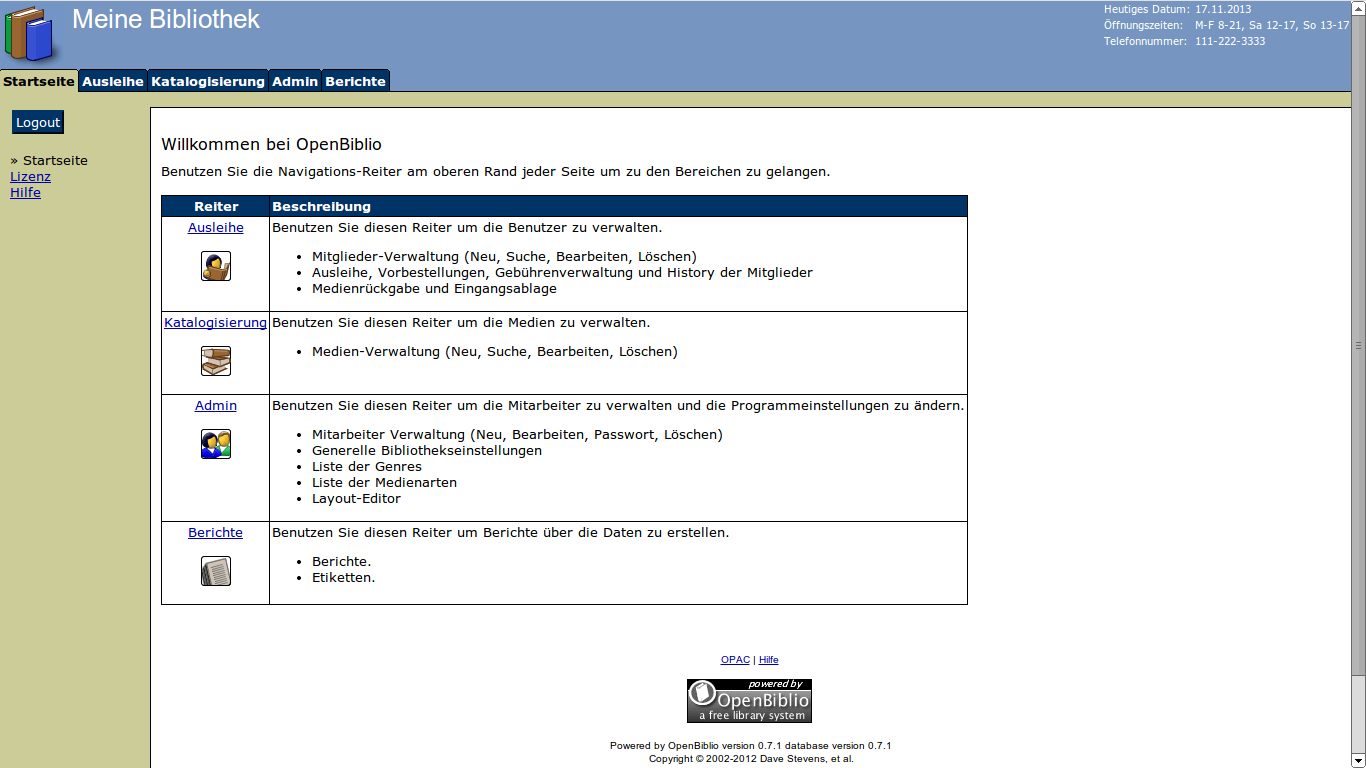
\includegraphics[width=1\textwidth]{OpenBiblio/startseite_loggedin.png}
\label{startseite-openbiblio}
\end{figure}
\\
Die Funktionen werden in vier Reiter zusammengefasst: \emph{Ausleihe}, \emph{Katalogisierung}, 
\emph{Admin} und \emph{Berichte}. Siehe Abbildung \ref{startseite-openbiblio}\\
\\
\begin{figure}[h]
\caption{Ausleihe in OpenBiblio}
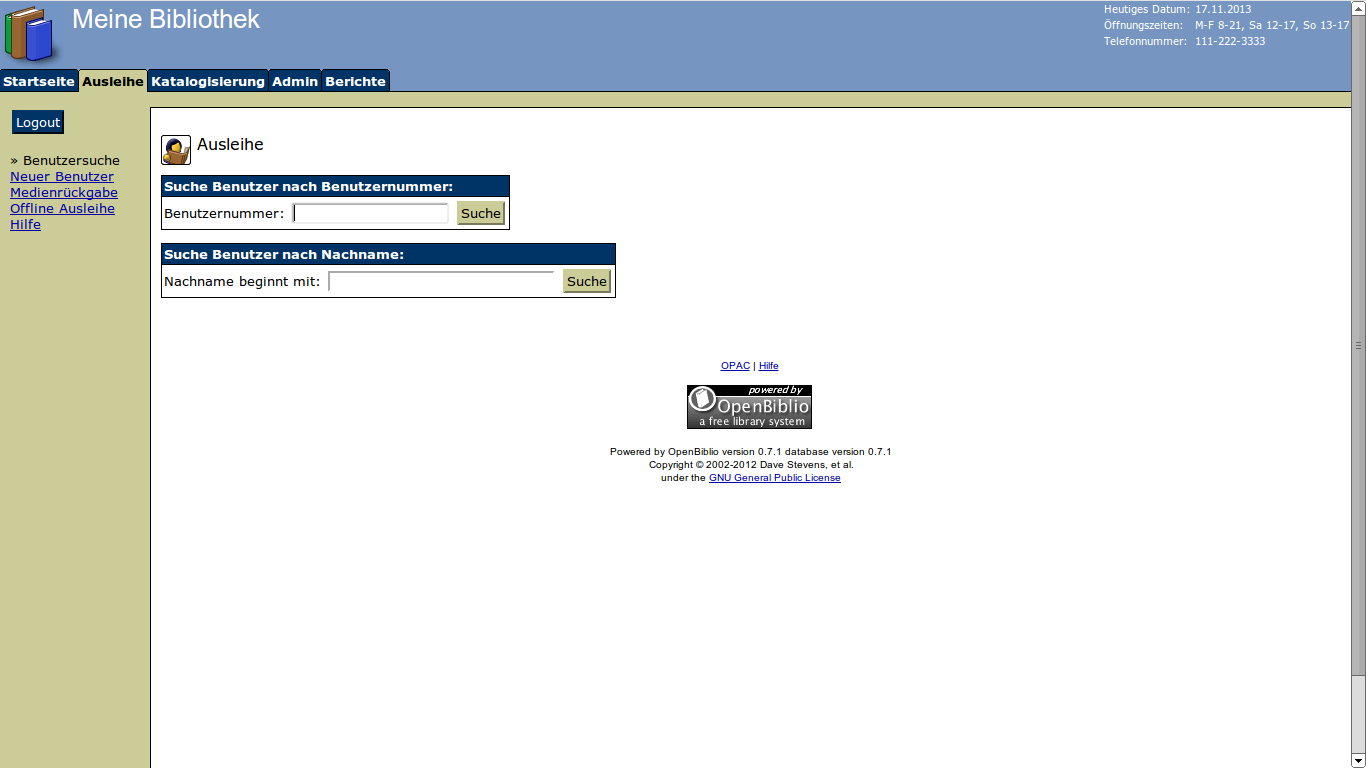
\includegraphics[width=1\textwidth]{OpenBiblio/reiter_ausleihe.png}
\label{ausleihe-openbiblio}
\end{figure}
\\
Auflistung aller Funktionen vom Reiter \emph{Ausleihe}:
\begin{itemize}
	\item Benutzersuche nach Nummer(ID) oder Nachname
	\item Neuen Benutzer erstellen
	\item Medienrückgabe
	\item Offline Ausleihe
	\item Mitglieder-Verwaltung:
	\begin{itemize}
		\item Neu, Suche, Bearbeiten, Löschen von Benutzern
		\item Detailansicht Benutzer, Ausleihliste, Benutzerinfos, Vorbestellen, Vorbestellliste
	\end{itemize}
\end{itemize}
\newpage
\begin{figure}[h]
\caption{Katalogisierung in OpenBiblio}
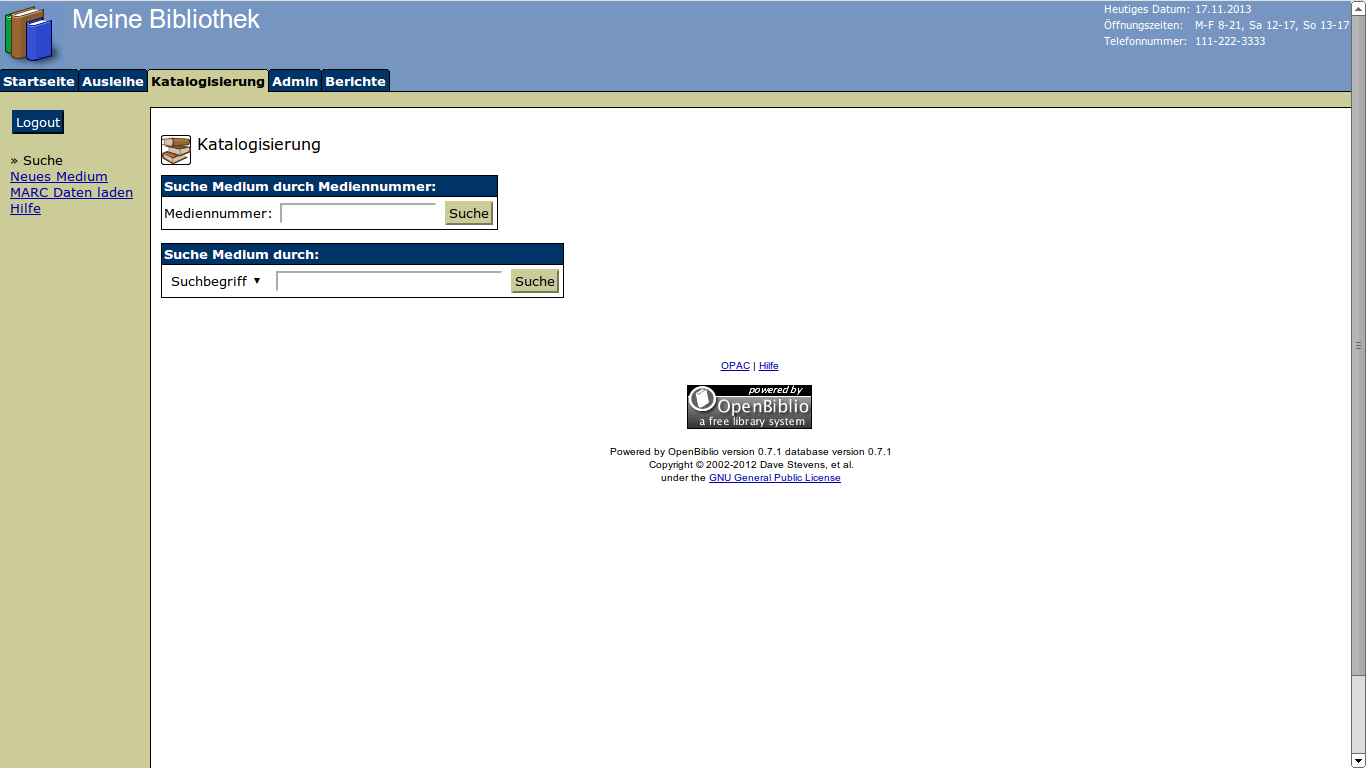
\includegraphics[width=1\textwidth]{OpenBiblio/reiter_katalogisierung.png}
  \label{katalogisierung-openbiblio}
\end{figure}
Funktionen im Reiter \emph{Katalogisierung}:
\begin{itemize}
	\item Mediensuche
	\item Mediendetailanischt:
	\begin{itemize}
		\item Medium bearbeiten
		\item Neues Exemplar hinzufügen
		\item Ausleihhistorie anzeigen
		\item Vorbestellungen anzeigen
		\item Medium löschen
		\item Ähnliches Medium hinzufügen
	\end{itemize}
	\item Hinzufügen, Suchen, Bearbeiten und Löschen von Medien
\end{itemize}
\newpage
\begin{figure}[h]
\caption{Adminbereich von OpenBiblio}
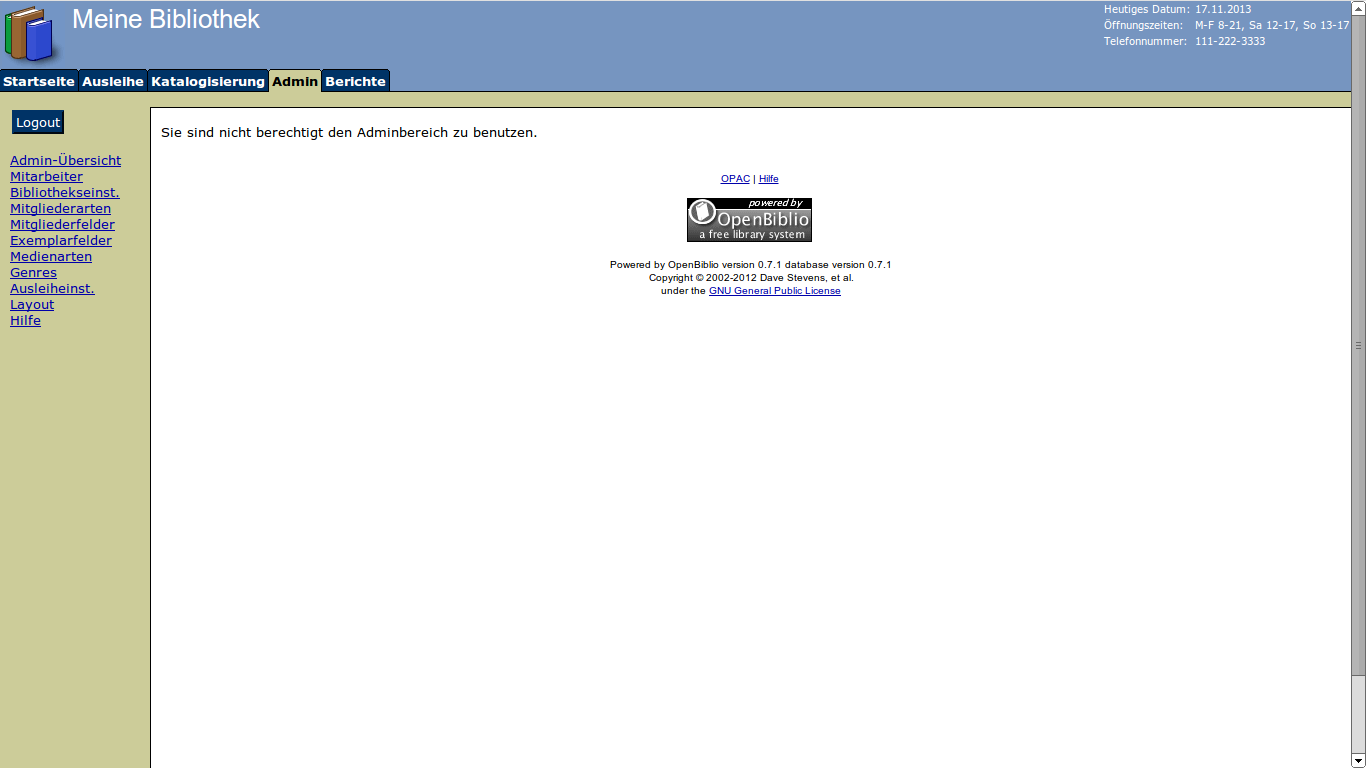
\includegraphics[width=1\textwidth]{OpenBiblio/reiter_admin.png}
  \label{admin-openbiblio}
\end{figure}
Funktionen im Reiter \emph{Admin} (Anmerkung: Diese Funktionen sind in der Testversion
nicht zugänglich! ):\\
\begin{itemize}
	\item Mitarbeiter verwalten, neu, bearbeiten, löschen
	\item Generelle Einstellungen
	\item Mitgliederarten
	\item Mitgliederfelder
	\item Exemplarfelder
	\item Ausleiheinstellungen
	\item Liste der Genres
	\item Liste der Medienarten
	\item Layout-Editor
\end{itemize}
\newpage
\begin{figure}[h]
\caption{Berichte in OpenBiblio}
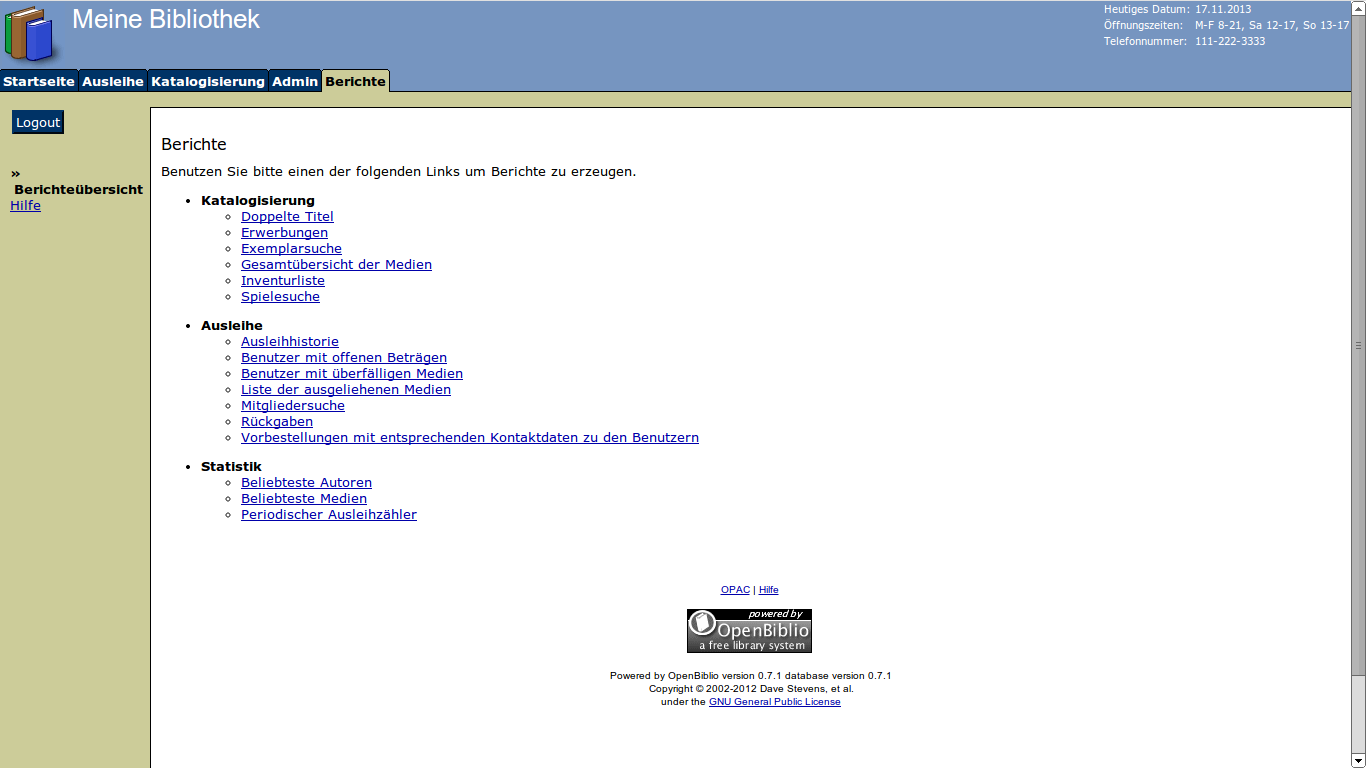
\includegraphics[width=1\textwidth]{OpenBiblio/reiter_berichte.png}
  \label{berichte-openbiblio}
\end{figure}
Funktionen im Reiter \emph{Berichte}:\\
\begin{itemize}
	\item doppelte Titel anzeigen
	\item Erwerbungen anzeigen
	\item Exemplarsuche
	\item Gesamtübersicht
	\item Inventurliste (alle Bücher nach Kriterium auflisten)
	\item Spielesuche
	\item Statistiken anzeigen:
	\begin{itemize}
		\item  Autoren
		\item Medien
		\item Ausleihungen
	\end{itemize}
	\item Benutzer mit offenen Beträgen anzeigen
	\item Benutzer mit überfälligen Medien anzeigen
	\item Liste der ausgeliehenen Medien
	\item Vorbestellungsliste
	\item Mitgliedersuche
	\item Rückgabeliste
\end{itemize}
Außerdem gibt es noch eine Hilfe:\\
\begin{figure}[h]
\caption{Hilfe in OpenBiblio}
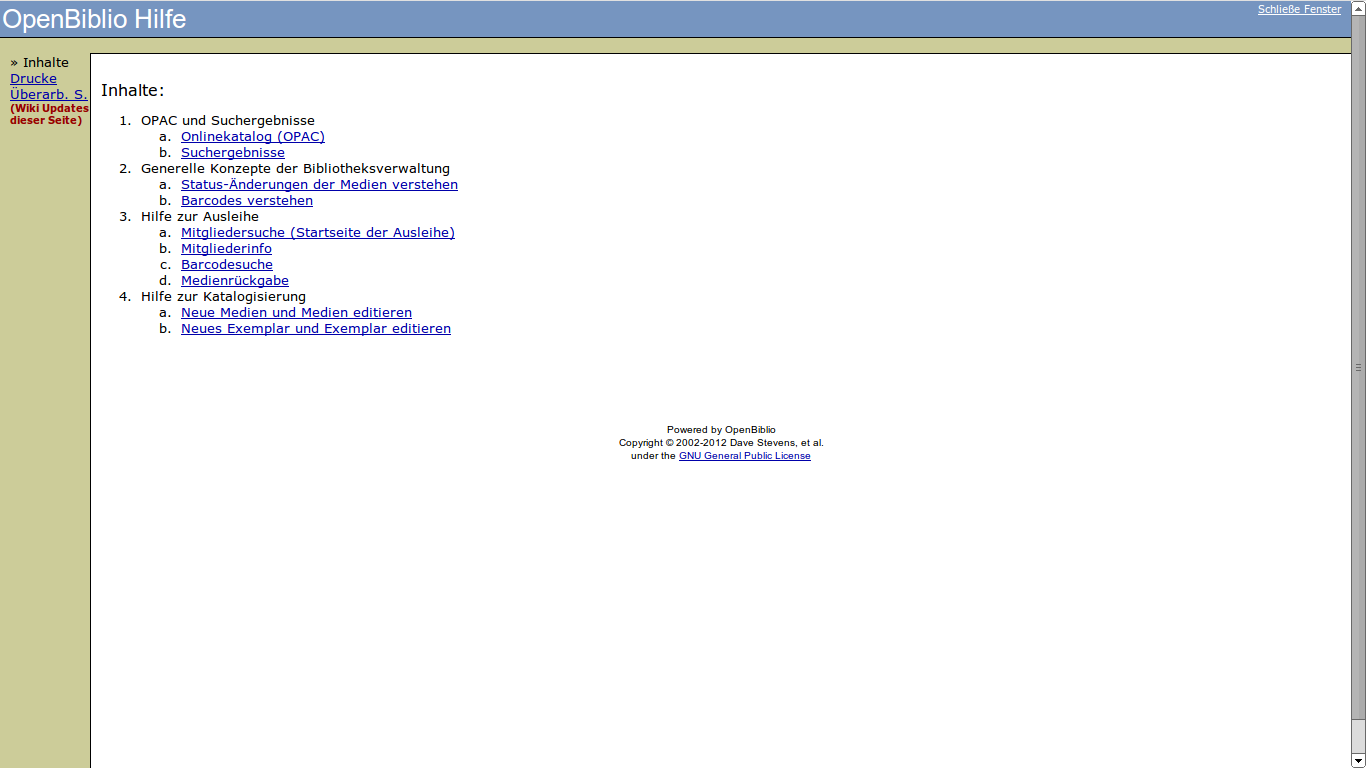
\includegraphics[width=1\textwidth]{OpenBiblio/hilfe.png}
  \label{hilfe-openbiblio}
\end{figure}

\subsection{Produktperspektive (Sebastian, Tim, Daniel)}
  
\subsubsection{Systemschnittstellen}


  Grundsätzlich wird ein bestehendes Computersystem (nebst typischen Ein- und Ausgabegeräten) 
  mit einem Betriebssystem vorausgesetzt, das mit den notwendigen Schnittstellen wie z.B. dem 
  Datenim- und -export umgehen kann.
  
  \textbf{CSV-Im-/Export:}\\
  Es gibt eine Funktion, mithilfe dieser CSV-Dateien importiert werden können. Diese kann nur vom 
  Administrator benutzt werden. Die Bücher werden anschließend in der Datenbank der Bibliothek 
  vorhanden sein. \\
  Es ist auch möglich, CSV Dateien zu exportieren, welche dann abgespeichert werden.

\subsubsection{Benutzerschnittstelle}

Als Schnittstelle zwischen Benutzer und Softwaresystem dient eine Internetseite, dessen Oberfläche 
seiner GUI als Screenshot unten dargestellt ist. \\
Die GUI weist je nach Benutzerrechten unterschiedliche Funktionalitäten auf, da es ein Unterschied ist, 
ob sich ein Ausleiher ins System einloggt oder ein Administrator. \\
Der Benutzer des Systems kann somit über einen Webbrowser mithilfe der typischen Eingabegeräte wie 
Tastatur und Maus auf diese Funktionen zugreifen und somit mit dem System interagieren. \\
Als Ausgabegerät dient selbstredend ein handelsüblicher Monitor, der in puncto Auflösung oder Größe 
keine besonderen, sondern nur minimalen Anforderungen (typischerweise mindestens 640x480 Pixel) 
genügen muss, sowie die Möglichkeit, einen Drucker einzusetzen, um beispielsweise eine Liste 
auszudrucken. \\
Ausgabeinteraktionsmechanismen sind in erster Linie Text sowie wenige Grafiken. 

\subsubsection{Hardwareschnittstellen} \label{hardware}
Das Softwaresystem besitzt als Schnittstelle zur Hardware das Betriebssystem des Computers bzw. des 
Smartphones. \\
  Es sind keine über minimale Anforderungen in Bezug auf RAM
  \footnote{RAM = Random Access Memory = Hauptspeicher des Computers}, Festplattenspeicher, 
  Prozessoren oder sonstigen Hardwarespezifika hinaus erforderlich. Somit wird die Software auch auf 
  älteren, internetfähigen Computersystemen laufen. \\
 
\subsubsection{Softwareschnittstellen} \label{software}

Unser System wird grundsätzlich plattformunabhängig laufen. Voraussetzung ist, dass das Java Runtime 
Environment sowie das Hibernate Framework (siehe Tabelle am Ende von Punkt \ref{Tabelle}) installiert 
ist. Für die App muss Android installiert sein. \\

   \textbf{Computer:}\\
  Unser System soll auf einem Web-Browser laufen. Dabei sollte das System auf Windows laufen, welches 
  die verwendete Plattform des Kunden ist. Dabei ist wichtig, dass alle Betriebssysteme von Windows 
  2000 bis Windows 8 unterstützt werden, da der Kunde Windows 2000 verwendet. Ebenfalls sollte das 
  System Linux und MacOS unterstützen. \\
  
  \textbf{Smartphone:}\\
  Unser System unterstützt nur Geräte, auf denen Android läuft. Dabei muss  die Version 2.3 oder höher 
  vorliegen, da somit der größte Teil der Android Geräte verwendet werden kann.\\
Im Folgenden dient eine Tabelle der Veranschaulichung von erforderlichen bzw. verwendeten Softwarekomponenten nebst 
Version.  \\ 

\label{Tabelle}
  \begin{tabular}{|l|l|l|l|}\hline
    \textbf{Name} & \textbf{Version} & \textbf{Hersteller} & \textbf{Quelle} \\\hline
    Java Runtime & 6 Update 37 & Oracle & \url{http://java.com/} \\\hline
    Hibernate & 4.3.0.Beta1 Release& JBoss Community &  
   \url{http://www.hibernate.org/}\\\hline
    Android & 2.3 oder höher & Open Handset Alliance & \url{http://www.android.com/} \\\hline
    JSON & 5.0 Release 8 & - & \url{http://json.org/} \\\hline
    REST & - & - & - \\\hline
    Primfaces & 4.0 & - & \url{http://www.primefaces.org/} \\\hline
  \end{tabular}
  

\subsubsection{Kommunikationsschnittstellen}

Unsere App muss eine Möglichkeit der Kommunikation mit dem Server haben, da sie in der Lage sein wird, z.B. Bewertungen abzuschicken. \\
Die Bandbreite des Servers muss dabei nicht so groß sein, da keine hohen Datenmengen ausgetauscht werden. \\ 
Es ist aber ein TCP/IP-Protokoll nötig, da die Serverapplikation öffentlich erreichbar sein wird.

\subsubsection{Speicherbeschränkung}
Wie schon im Punkt \ref{hardware} beschrieben, gibt es keine Speicherbeschränkungen. Ein PC, auf dem, 
wie beim Kunden, Windows 2000 läuft, kann also problemlos verwendet werden. Das Softwaresystem 
beansprucht nicht viele Ressourcen in puncto RAM oder Festplattenspeicher.

\subsubsection{Operationen (Betriebsmodi)}
  
  Das System wird vier verschiedene Betriebsmodi umfassen. Zum einen der Administratorenmodus, in dem man grundlegende Einstellungen verändern kann sowie einen Vollzugriff auf das System hat. So ist es möglich, Bibliothekare zu löschen oder hinzuzufügen. \\
Zum anderen der Bibliothekarmodus, der den Mitarbeitern der Bibliothek ermöglicht, auf fast alle Funktionen des Administrators zuzugreifen, die für den Leser oder Gast natürlich nicht vorgesehen sind (Medienbestandsverwaltung, Ausleiher sperren usw.).\\
Im Lesermodus sind nur die Funktionen zugelassen, die für Ausleiher angemessen sind (Im Bestand suchen, Medien vormerken und rezensieren usw.). \\
Im Gästemodus kann man schließlich nur noch die Publikationsliste einsehen und Buchdetails, nicht jedoch Medien bewerten oder vormerken.

\subsubsection{Möglichkeiten der lokalen Anpassung}

 Es handelt sich bei dem System um ein lauffähiges Gesamtpaket. Es muss keine Datenbank o.Ä. eingerichtet werden. Lediglich eine IP-Adresse muss eingerichtet werden. Somit ist die App so lauffähig und es ist keine lokale Anpassung nötig.


\subsection{Anwendungsfälle}
  {\em Auflistung und kurze Beschreibung aller relevanten
  Anwendungsfälle. Dies soll einen Überblick über alle Anwendungsfälle
  geben, die in 3.2 detailliert beschrieben werden.}
  
\begin{itemize}
  \item \textbf{1. Programm starten}\\
  Website wird aufgerufen/ App wird gestartet. 
  \item \textbf{2. Benutzer anmelden}\\
  Ein Benutzer meldet sich an.
  \item \textbf{3. Benutzer abmelden} \\
  Ein Benutzer meldet sich ab.
  \item \textbf{4. Start anzeigen}
  Startseite wird mit dem "Start-Button"         
  aufgerufen.
  \item \textbf{5 Leserprofil anzeigen}
  Profil des Lesers wird mithilfe des 
  Buttons "Profil" angezeigt.
  \item \textbf{6 Vormerkung bearbeiten}
  Eigene in der Profilsicht angezeigte     
  Vormerkungen werden bearbeitet.
  \item \textbf{7. Publikationen anzeigen}
  Liste der Publikationen wird mithilfe
  des Buttons "Publikationen" angezeigt.
  \item \textbf{8. Medium hinzufügen}
  Neues Medium kann durch klicken auf 
  "Medium hinzufügen" und 
  \item \textbf{9. Medium ändern}
  \item \textbf{10.Medium löschen}
  \item \textbf{11. CVS-Import}
  Importieren einer CVS-Datei für 
  die Publikationen.
  \item \textbf{12. CVS-Export}
  Exportieren einer CVS-Datei für die
  Publikationen.
  \item \textbf{13. Buch suchen}
  In das 'Suchen-Textfeld' wird 
  der Titel des gesuchten Buches eingegeben.
  \item \textbf{14. Einzelnes Buch anzeigen/ Detailansicht}
  Mithilfe des Klicks auf den Pfeil, wird 
  die Detailsicht aufgerufen.
  \item \textbf{15. Medium bewerten}
  Ein Buch wird in der Detailansicht 
  bewertet.
  \item \textbf{16. Medium ausleihen}
  Bibliothekar leiht Leser ein oder 
  mehrere Medien aus.
  \item \textbf{17 Mediumrückgabe}
  Bibliothekar nimmt zurückgegebene
  Medien durch einscannen a, Ausleihablauf
  wird kontrolliert und Medien und Leser 
  werden auf den neusten Stand gebracht.  
  \item \textbf{18 Medium rezensieren}
  Leser kann in der Detailansicht 
  das Buch kommentieren.
  \item \textbf{19. Medium vormerken}
  Medien können in der Publikationsübersicht    
  vorgemerkt werden.
  \item \textbf{20. Rezension freischalten}
  Rezension muss vor Veröffentlichung von einem
  Bibliothekar freigeschaltet werden.
  \item \textbf{21. Leserliste anzeigen}
  Durch klicken auf 'Leser' wird die Leser-  
  übersicht oder Liste angezeigt.
  \item \textbf{22. Leser hinzufügen}
  Nach Klicken auf 'Leser hinzufügen'
  kann ein neuer Leser eingerichtet
  werden.
  \item \textbf{23. Leser ändern}
  Leserdaten können von einem 
  Bibliothekar geändert werden.
  \item \textbf{24. Leser löschen}
  Ein Leserprofil kann von einem Bibliothekar 
  gelöscht werden.
  \item \textbf{25. CVS-Import}
  Importieren einer CVS-Datei für 
  die Leserliste
  \item \textbf{27. CVS-Export}
  Exportieren einer CVS-Datei für 
  die Leserliste.
  \item \textbf{28. Einzelnen Leser anzeigen/  
  Detailansicht}
  Durch Klicke auf den Pfeil wird die 
  Detailansicht angezeigt.
  \item \textbf{29  Leser sperren}
  Leser kann von einem Bibliothekar gesperrt
  werden.
  \item \textbf{30. Leser suchen}
  Mithilfe des 'Suchen-Textfeldes' kann
  in der Leserübersicht nach einem Leser 
  gesucht werden.
  \item \textbf{31. Administration öffnen}
  Durch Klicken auf den Button Administration 
  wird die Übersicht der Administration 
  angezeigt.
  \item \textbf{32. Bibliothekarliste anzeigen}
  Bibliothekarliste kann durch den Admin 
  aufgerufen werden.
  \item \textbf{33. Bibliothekar hinzufügen}
  Der Admin kann in dem Bereich Administration
  durch klicken des Buttons 'Bibliothekar
  hinzufügen' einen neuen Bibliothekar 
  einrichten.
  \item \textbf{34. Bibliothekar löschen}
  Der Admin kann einen Bibliothekar löschen.
  \item \textbf{35. Bibliothekar ändern}
  Profildaten eines Bibliothekars können durch 
  den Admin geändert werden.
  \item \textbf{36. Statistiken anzeigen}
  Statistiken können im Bereich der       
  Administration durch den Button
  'Statistiken anzeigen' aufgerufen werden.
  \item \textbf{37. Mahnungsliste anzeigen}
  Im Bereich der Administration kann die
  Mahnungsliste durch betätigen des 
  entsprechenden Butons angezeigt werden.
  \item \textbf{38. Mahnungsliste drucken}
  In der Anzeige der Mahnungsliste kann durch 
  den Button 'Drucken' die Mahnungsliste
  ausgedruckt werden.
  \item \textbf{39. Mahnungsdetails anzeigen}
  Durch Klicken auf den Pfeil in der 
  Übersicht der Mahnungsliste, können Details
  der Mahnungen eines bestimmten Leser 
  angezeigt werden.
  \item \textbf{40. Startseite bearbeiten}
  Die Startseite kann mit Nachrichten und
  Meldungen beschrieben werden.
  \item \textbf{41. Abgabedaten und Mahngebühren bearbeiten}
  Bibliothekare können Abgabedaten und
  Mahngebühren individuell anpassen.
 \end{itemize}


\subsection{Charakteristika der Benutzer (Daniel)}


\begin{table}[htbp]
\caption{Benutzer}
\label{benutzer}
\begin{tabular}{|p{2,5cm}||p{2,8cm}|p{2,8cm}|p{2,8cm}|p{2,8cm}|}
\hline 
\textbf{Name(fiktiv)} & Bert Bib & Arnold Admin & Silke Schüler & Bart Besucher\\ \hline
\textbf{Bild(fiktiv)} & 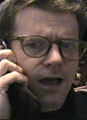
\includegraphics[scale=1]{bib.jpg} & 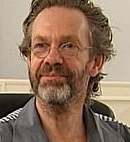
\includegraphics[scale=0.6]{admin.jpg} & 
\includegraphics[scale=0.45]{reg.jpg} & 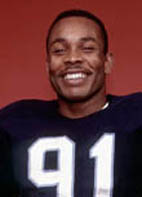
\includegraphics[scale=0.45]{unreg.jpg} \\ \hline
\textbf{Rolle} & Bibliothekar & Administrator & Leiherin & uregistrierter Leiher \\ \hline
\textbf{Beruf} & Bibliothekar & Bibliothekar & Schülerin & Anwalt\\ \hline
\textbf{Alter} & 39 & 56 & 16 & 34\\ \hline
\textbf{Ziel} & Bibliothek verwalten & System verwalten & Bücher ausleihen & Bücher ausleihen \\ \hline
\textbf{Verwendung der Software} & Bücher und Nutzer verwalten & System und Bibliothekare verwalten 
& Bücher suchen, ausleihen etc. & keine\\ \hline
\end{tabular}
\end{table}

\textbf{Bert Bib:}\\
Bert Bib ist ein Bibliothekar in der Bibliothek und arbeitet dort. Er wohnt in Bremen und ist 39 Jahre alt. Er fährt jeden Morgen mit Auto zur Arbeit und braucht dafür 25 Minuten. Er ist Verheiratet und hat 2 Kinder, welche beide männlich sind und zur Grundschule gehen. Der Ältere geht in die 4.Klasse und der jüngere in die 1.Klasse. Er ist ein großer Fussballfan und sein Lieblingsverein ist Hannover 96, da er in Hannover geboren und aufgewachsen ist. Er arbeitet bereits seit 13 Jahren als Bibliothekar und ist seit 8 Jahren an der Schule Rockwinkel beschäftigt. Er ist mit dem momentanen System unzufrieden, da der Ausleihvorgang sehr aufwändig ist. Von der neuen Software erhofft er sich eine leichtere und schnellere Verwendung um die Bibliothek zu verwalten und Bücher auszuleihen. \\

\bigskip

\textbf{Arnold Admin:}\\
Arnold Admin ist ein Lehrer an der Schule Rockwinkel und ist als Administrator für die Software zuständig. Er hat Grundkenntnisse in Informatik und kennt sich guten mit Computern aus. Er lehrt Mathematik und Physik an der Oberschule. Er ist 56 Jahre alt und wohnt auch in Bremen. Er fährt jeden Tag mit Bus zur Schule und braucht dafür 15 Minuten. Arnold war dreimal verheiratet und ist zweimal geschieden. Er hat zwei Töchter aus erster Ehe, welche bereits Berufstätig sind. Aus der aktuellen Ehe hat er einen Sohn, welcher 12 Jahre alt ist und in die 7. Klasse geht. Er liebt Bücher über alles, weshalb er sich auch als Administrator für die Bibliothek gemeldet hat. Er ist auch dafür zuständig Bibliothekare einzustellen und zu entlassen. Die Software wird er benutzen, um neue Bibliothekare zu registrieren und zu löschen. Er muss zudem auch wöchentlich die Dateien sichern und ein Back-up machen.\\

\bigskip

\textbf{Silke Schüler:}\\
Silke Schüler ist eine Schülerin der Oberschule Rockwinkel und besucht die 11.Klasse. Sie ist eine durchschnittliche Schülerin, welche beliebt unter ihren Klassenkameraden ist. Sie hat einen Freund, welcher zur Zeit eine Ausbildung macht. Sie wohnt in Bremen bei ihren Eltern und ist 16 Jahre alt. Zur Schule fährt sie immer mit dem Fahrrad und braucht dafür 10 Minuten. Sie geht am Wochenende gerne in Diskotheken oder trifft sich mit ihren Freunden. Sie lernt am liebsten mit Fachbüchern über das jeweilige Thema und ist deshalb öfter mal in der Bibliothek anzutreffen. Sie wünscht sich schon seit längeren eine App für die Bibliothek, da sie viel Zeit mit ihren Smartphone verbringt und so schnell nach Büchern suchen kann. Da sie sehr vergesslich ist, ist für sie auch ein Vorteil, dass sie über die App schnell nachgucken kann, wann sie die Bücher abgeben muss.\\

\bigskip

\textbf{Bart Besucher:}\\
Bart Besucher ist 34 Jahre alt und arbeitet als Anwalt. Er wohnt in Delmenhorst und ist momentan noch verheiratet, lebt aber getrennt von seiner Frau. Er hat einen Sohn, welcher noch in den Kindergarten geht und 5 Jahre alt ist. Er ist früher an der Oberschule Rockwinkel zur Schule gegangen, weshalb er die Bibliothek noch regelmäßig besucht. Die Software würde für ihn eine leichtere Suche bedeuten, indem er auch schon zu Hause Bücher suchen kann, da er sehr beschäftigt ist und wenig Zeit hat.\\

\subsection{Einschränkungen}
\label{sec:Einschraenkungen}
Im Folgenden listen wir die Mindestanforderungen des Produkts welche ebenfalls der Webseite der Veranstaltung Software Projekt 2 der Universität Bremen im Wintersemester 2013/14 entnommen werden können\footnote{\url{http://www.informatik.uni-bremen.de/st/Lehre/swpII_1314/mindestanforderungen.html}}:

\begin{itemize}

\item Unterschiedliche Medientypen werden unterstützt.
\item Exemplare werden unterstützt.
\item Standorte der Medien innerhalb der Bibliothek werden unterstützt.
\item Gast, Leser, Bibliothekare und Administratoren werden als Benutzergruppen unterschieden.
\item Alle Nutzer außer Gäste müssen sich authentifizieren.
\item Veränderungen der Daten der Bibliothek werden protokolliert (z.B. bei Veränderungen beim Verleihen, der Rückgabe, Verlängerung, Mahnung,...) und können durch Bibliothekare eingesehen werden.
\item Medien können von den Bibliothekaren hinzugefügt, geändert und gelöscht werden.
\item Medien können in Kategorien einsortiert werden und neue Kategorien erstellt werden.
\item Inaktive Leser werden zur Löschung vorgeschlagen.
\item Bibliothekare verleihen Medien.
\item Der automatisch festgelegte Rückgabezeitraum berücksichtigt die Öffnungszeiten, die der Bibliothekar festlegt.
\item Individuelle Abgabedaten und Mahngebühren können vom Bibliothekar festgelegt werden.
\item Bibliothekar kann Verlängerungswünsche der Leser berücksichtigen.
\item Leser können Medien vormerken; Bibliothekare sehen alle Vormerkungen, Leser ihre eigenen.
\item Bibliothekare können ausgeliehene Bücher wieder entgegennehmen.
\item Bibliothekare richten Leser ein, können sie ändern und löschen.
\item Bibliothekare können mindestens den letzten Ausleiher einsehen.
\item Bibliothekare haben eine Übersicht über verliehene Bücher, Versäumnisse und fällige Mahngebühren.
\item Mahngebühren und Ausleihfristen können sich je nach Medientyp unterschiedlich von 
\item Bibliothekaren festgelegt werden.
\item Bibliothekare können Statistiken einsehen zu:
\begin{itemize}
\item Ausleihzeiträumen
\item Verteilung der Ausleihen auf Leser
\item Häufig und selten ausgeliehenen Medien
\item Vormerkzeiten
\item Bewertungen
\end{itemize}
\item Die Startseite kann redaktionell bearbeitet werden und aktuelle Nachrichten enthalten.
\item Leser können Rezensionen zu Medien schreiben, die aber erst von Bibliothekaren freigeschaltet werden müssen.
\item Ein Administrator richtet neue Bibliothekare ein, löscht sie oder verändert deren Stammdaten.
\item Versionierte Backups und Restore aller Daten sind im laufenden Betrieb und automatisch möglich.
\item Leser können über eine Android App bzw. über eine für mobile Geräte optimierte Website auf das System zugreifen.
\item Leser sehen ihre ausgeliehenen Medien, Rückgabefristen und Mahngebühren.
\item Leser können Nachrichten zu Rückgabefristen, Mahngebühren sowie verfügbare vorgemerkte Medien erhalten.
\item Leser können Verlängerungswünsche einreichen.
\item Ein Leser kann bestimmen, ob seine Ausleihhistorie gespeichert und für ihn einsehbar ist.
\item Leser können Medien bewerten.
\item Leser können Rezensionen zu Medien schreiben.
\item Neueste freigeschaltete Rezensionen werden in einer Übersicht angezeigt.


\end{itemize}

\subsubsection{Technische Rahmenbedingungen}
\begin{itemize}

\item Softwareergonomische Prinzipien werden umgesetzt.
\item Die Funktionalitäten aller Nutzer (Administratoren, Bibliothekare, Leser, Gäste) können über einen Web-Browser verwendet werden.
\item Die Software funktioniert auf der Hard- und Softwareplattform des Kunden (Windows) sowie unter Linux und MacOS.
\item Als Application-Server wird GlassFish 3.1 benutzt.
\item Es muss eine relationale Datenbank für die serverseitige Persistenz benutzt werden:
\begin{itemize}
\item Persistenz-Frameworks sind erlaubt (z.B. JPA), aber dann ist eine deklarative Verwendung von SQL-ähnlichen Abfragen verlangt.
\item Verwendung leichtgewichtiger DBMS (z.B. Derby, SQLite) ohne echte Serverinstallation ist vorgeschrieben.
\end{itemize}
\item Verwendung und Abgabe eines Build-/Installationsskriptes, damit die Anwendung einfach installiert und aus den Quellen gebaut werden kann. Alle notwendigen Installations- und Konfigurationsschritte sind dokumentiert.
\item Eventuell benutzte Fremdbibliotheken dürfen für den Einsatz in Forschung und Lehre keine Beschränkungen (Geld, Benutzung, ...) aufweisen.
\item Quelltext in Deutsch oder Englisch dokumentiert. Gleiches gilt für Variablen- und Klassennamen. Alle anderen Dokumente in Deutsch.
\item Die Implementierungssprache ist Java 5 oder höher (weitere zulässige Sprachen in geringem Umfang sind: HTML, XML und JavaScript).
\end{itemize}

\newpage
\subsubsection{Gesetzliche Rahmenbedingungen}

Hier gilt in erster Linie das deutsche Recht. Um genau zu sein kommen hier das Datenschutzgesetz\footnote{\url{http://www.gesetze-im-internet.de/bdsg_1990/}} und das Urheberrecht\footnote{\url{http://www.gesetze-im-internet.de/urhg/}} zum tragen. Verfahrensrechtliche Vorkehrungen um die Datensicherheit\footnote{\url{http://www.gesetze-im-internet.de/bdsg_1990/__9.html}} zu gewährleisten sind von dem Kunden zu treffen. Der Kunde wird von der Software hinsichtlich der technischen Vorkehrungen insofern unterstützt, dass der Zugriff auf die Daten und der Zugang auf das Administrationstool passwortgeschützt ist.
Hinsichtlich des Urheberrechts ist besonders auf die Regelung für Computerprogramme\footnote{\url{http://www.gesetze-im-internet.de/urhg/BJNR012730965.htm\#BJNR012730965BJNG004201377}} zu achten.
 
\subsubsection{Sicherheitskritische Aspekte}

Um das deutschen Datenschutzgesetz einzuhalten muss der Kunde weitere Maßnahmen treffen. Diese sind nicht entscheident für die Entwicklung der Software und liegen in der Verantwortung des Kunden.

\subsection{Annahmen und Abhängigkeiten}

Bis zur Auslieferung der Software wird sich der Kunde nicht ändern. Die Anforderungsspezifikation dient 
als eine Art Vertrag mit dem Kunden. Deshalb ist davon auszugehen, dass nach der Abgabe der 
Anforderungsspezifikation keine zusätzlichen Anforderungen hinzukommen. \\
Abgabetermine haben Deadlines und sind somit strikt einzuhalten.\\

Des Weiteren wird davon ausgegangen, dass sich die Nutzer der Software zwar mit dem System 
eingehend auseinandersetzen. Es wird jedoch auch für den ungeübten Nutzer leicht möglich sein, dieses 
zu verwenden. Der jeweilige Nutzer sollte zumindest schon mal mit einem Computer gearbeitet haben.\\

Zu Hardware- und Software-Abhängigkeiten geben die Punkte \ref{hardware} (Hardwareschnittstellen) 
und \ref{software} (Softwareschnittstellen) hinreichend Aufschluss.
 
\subsection{Ausblick}
\nurlangversion

  {\em Beschreibt hier knapp, welche Änderungen und Erweiterungen
  zukünftig (d.h.\ nach Auslieferung des Systems) zu erwarten sind.
  Diese Information ist wichtig für den Entwurf, um mögliche
  Änderungen frühzeitig im ersten Entwurf berücksichtigen zu können.
  Der Entwurf kann dann so gestaltet werden, dass die zukünftigen
  Anforderungen leicht realisierbar sind. Die zukünftigen
  Anforderungen sollten realistisch sein, ansonsten könnte ein unnötig
  allgemeiner und damit zu komplizierter Entwurf die Folge sein.  Auch
  dieser Abschnitt ist im IEEE-Standard nicht vorgesehen -- zumindest
  nicht explizit in Form eines eigenständigen Abschnitts. Dennoch
  handelt es sich um wertvolle Information, von der der Entwurf
  profitieren kann.}
  

\section{Detaillierte Beschreibung}
\label{ch:DetaillierteBeschreibung}
{\em Die externen Schnittstellen werden grob in Abschnitt 2
  beschrieben.  Wenn die grobe Beschreibung dort nicht genügt, kann
  sie hier detaillierter ausgeführt werden (wie vom IEEE-Standard
  vorgesehen).}

\subsection{Datenmodell}
\begin{itemize}
 \item \textbf{1. Person:}\\
  Stellt die Oberklasse aller Nutzer, Bibliothekare oder 
  des Admins dar.

\item \textbf{2. Admin:}\\
Die Klasse Admin oder Administrator erbt von Person und kann mithilfe der    Assoziationsklasse '"Bearbeiten/Löschen/Hinzufügen"' die Profildaten eines
Bibliothekars entweder bearbeiten oder eine kompletten Bibliothekar löschen 
oder  neu einrichten.
 
\item \textbf{3. Bibliothekar:}\\
Die Klasse Bibliothekar erbt von Person und kann Rezensionen freischalten und
kann Daten von sowohl Leihobjekt, der Assoziationsklasse Ausleihe, als auch 
dem Nutzer bearbeiten. Zusätzlich ist Bibliothekar an der Ausleihe beteiligt.

\item \textbf{4. Nutzer:}\\
Auch der Nutzer erbt von Person und stellt den Leser dar, der sowohl Exemplare
ausleihen und vormerken bzw. reservieren, als auch das Leihobjekt bewerten und 
rezensieren kann.

\item \textbf{5. Leihobjekt:}\\
Die Klasse Leihobjekt stellt ein beliebiges Medium dar, welches in der 
Bibliothek vorhanden ist. Gleichzeitig ist sie die Oberklasse für Buch,
CD und noch eine Ebene weiter auch für Exemplar. Das Leihobjekt wird vom Nutzer
bewertet und rezensiert und vom Bibliothekar erstellt oder entweder bearbeitet 
oder gelöscht.

\item \textbf{6. Buch:}\\
Das Buch erbt von Leihobjekt und ist gleichzeitig eine mögliche Oberklasse
für Exemplar. Zusätzlich steht es mit der Klasse Buchreihe über eine Aggregation
in Verbindung. 

\item \textbf{7. Buchreihe:}\\
Die Klasse Buchreihe steht mit der Klasse Buch über eine Aggregation in Verbindung.
Eine Buchreihe kann beliebig viele Buchobjekte besitzen.
 
\item \textbf{8. CD:}\\
CD erbt ebenfalls von Leihobjekt und ist eine mögliche Oberklasse für Exemplar.

\item \textbf{9. Exemplar:}\\
Das Exemplar ist das Objekt, welches an den Nutzer verliehen und von diesem reserviert oder vorgemerkt wird. Es hat eine individuelle ID mit der bei der Rückgabe, Medien
eindeutig dem entsprechenden Nutzer zugeordnet werden kann. Exemplar erbt entweder von
der Klasse Buch oder von der Klasse CD, niemals beide oder keinem von beiden. Ein Exemplar ist also immer entweder eine CD oder ein Buch.

\item \textbf{10. Ausleihe:}\\
Die Assoziationsklasse Ausleihe stellt den Vorgang des Ausleihens dar.
Es beschreibt die Verbindung zwischen dem Nutzer, dem Bibliothekar und dem Exemplar, indem es unter anderem die ID des verliehenen Exemplars und die zu beachtende Frist 
als Variablen bekommt. 


\item \textbf{11. Reservierung/Vormerkung:}\\
Diese Assoziationsklasse bekommt das aktuelle oder gewünschte Datum der vom Nutzer getätigten Vormerkung oder Reservierung zugeschrieben.

\item \textbf{12. Bewertung:}\\
Die Assoziationsklasse Bewertung stellt die Bewertung eines Nutzers zu einem Leihobjekt dar. Zum Festhalten der Bewertungshöhe erhält die Klasse Bewertung
eine Integer-Variable 'Bewertung'.

\item \textbf{13. Rezensieren:}\\
Assoziationsklasse. Ein Nutzer kann über ein Leihobjekt eine Rezension schreiben, die allerdings vor der Veröffentlichung von einem Bibliothekar freigeschaltet werden muss. Sie bekommt eine String-Variable für den vom Nutzer verfassten Text und ein Boolean, ob die Rezension freigegeben wurde.

\item \textbf{14. Bearbeiten/Löschen/Hinzufügen:}\\
Eine Assoziationsklasse. Ermöglicht Bibliothekare diese drei Funktionen an den Klassen 
Leihobjekt, Ausleihe und Nutzer anzuwenden. Auch beschreibt sie Fähigkeit des Admins,
Bibliothekare zu bearbeiten, zu löschen oder hinzuzufügen.
\end{itemize}
 

  {\em Das Datenmodell im Kontext des Pflichtenhefts ist {\glqq}die
  Darstellung von Informationen und deren Beziehungen in einem
  fachlogischen Konzept{\grqq}. Es soll hier gezeigt werden, welche
  Einheiten für das existierende System relevant sind und welche
  Beziehungen zwischen diesen Einheiten gelten. Es handelt sich
  hierbei noch nicht um ein Datenbankschema oder eine Spezifikation
  von Klassen für die Implementierung (Entwurf), sondern um die
  Modellierung der realen Welt. Das Datenmodell ist leitend für den
  Entwurf (weil alles darin beschrieben sich auch in der Software 
  wiederfinden wird), aber nimmt den Entwurf nicht schon vorweg.
  
  Das Datenmodell soll als UML-Klassendiagramm angegeben werden.
  Wichtig ist hierbei die korrekte Verwendung der UML: Klassen,
  Attribute, Generalisierung, Assoziation, Aggregation, Komposition,
  Multiplizitäten. Außerdem sollte das Diagramm sinnvoll und gut
  lesbar sein. Dazu gehört weiterhin eine kurze Beschreibung des
  Modells mit ergänzenden Informationen, insbesondere wenn die
  Relationen durch ihren Namen nicht selbsterklärend sind. Gebt
  unbedingt ein Mengengerüst für die Daten an: Wie viele Instanzen der
  wichtigsten Klassen werden erwartet? Erwartet Ihr Änderungen im
  Datenvolumen in der Zukunft?}


\subsection{Anwendungsfälle}
\begin{figure}[htbp]
\caption{Startseite}
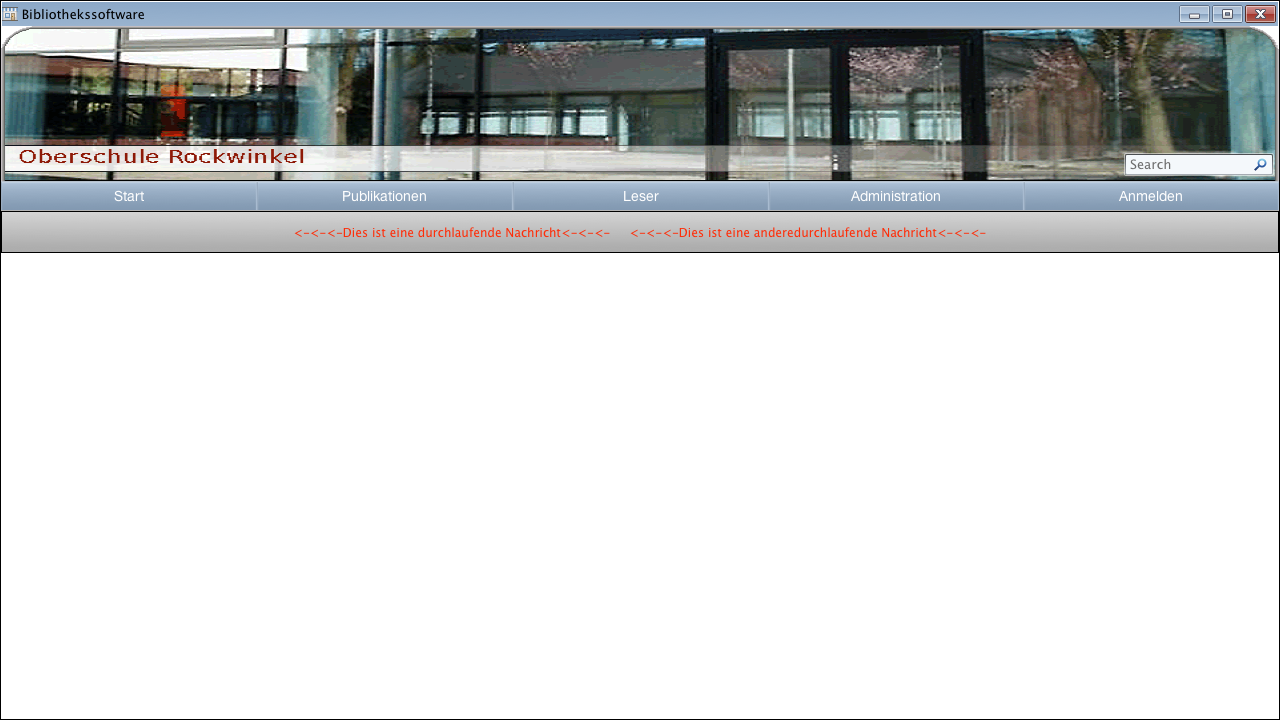
\includegraphics[width=1\textwidth]{WebApp-Screens/Startscreen-loggedOut.png}
  \label{startseite}
\end{figure}

\begin{table}[htbp]
\label{1}
\begin{tabular}{|l|p{10cm}|}
\hline 
\textbf{1} & \textbf{Programm starten} \\ \hline
\textbf{Akteure} & Bert Bib, Arnold Admin, Silke Schüler, Bart Besucher\\ \hline
\textbf{Ziel} & Der Akteur möchte das Programm starten  \\ \hline
\textbf{Vorbedingungen} & keine \\ \hline
\textbf{Regulärer Ablauf} & 
1. Der Akteur startet das Programm, indem er die URL aufruft \\
&2. Das Programm startet und zeigt die Startseite \\ \hline
\textbf{Varianten} & keine \\ \hline
\textbf{Nachbedingungen} & Das Programm ist gestartet und der Benutzer kann dieses nun verwenden\\ 
\hline
\textbf{Fehler-/Ausnahmefälle} & Server ist nicht erreichbar \\ \hline
\end{tabular}
\end{table}

\begin{figure}[htbp]
\caption{Loginscreen}
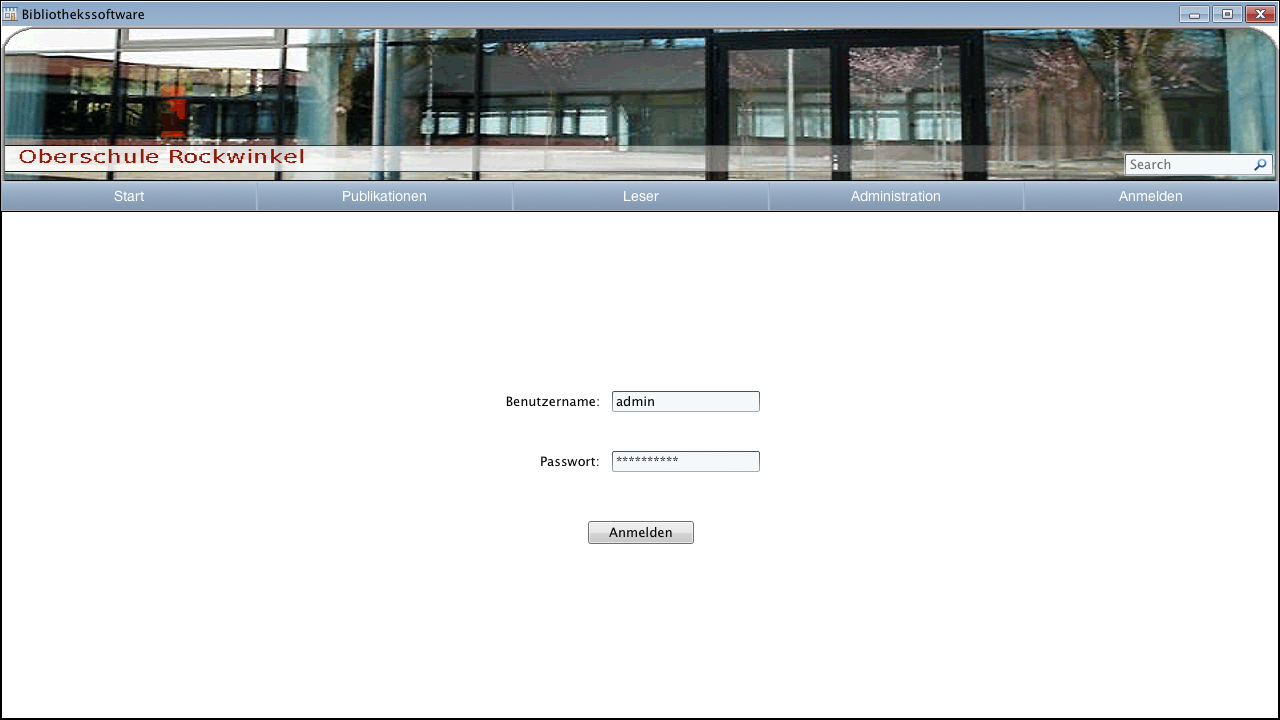
\includegraphics[width=1\textwidth]{WebApp-Screens/Loginscreen.png}
  \label{login}
\end{figure}

\begin{table}[htbp]
\label{2}
\begin{tabular}{|l|p{10cm}|}
\hline 
\textbf{2} & \textbf{Benutzer anmelden} \\ \hline
\textbf{Akteure} & Bert Bib, Arnold Admin, Silke Schüler, Bart Besucher\\ \hline
\textbf{Ziel} & Der Akteur möchte sich im System anmelden  \\ \hline
\textbf{Vorbedingungen} & Das Programm wurde gestartet  \\ \hline
\textbf{Regulärer Ablauf} & 
1. Bib gibt seinen Benutzernamen und sein Passwort ein \\
&2. Bert Bib drückt auf den Button anmelden\\
&3. Der Startbildschirm erscheint wieder und Bert Bib kann nun alle Funktionen eines Bibliothekars 
verwenden\\ \hline
\textbf{Varianten} & 
1. Arnold Admin gibt seinen Benutzernamen und sein Passwort ein \\
&2. Arnold Admin drückt auf den Button 'Anmelden'\\
&3. Der Startbildschirm erscheint wieder und Arnold Admin kann nun alle Funktionen eines 
Administrators verwenden\\  
& \\
&1. Silke Schüler gibt ihren Benutzernamen und ihr Passwort ein \\
&2. Silke Schüler drückt auf den Button 'Anmelden'\\
&3. Der Startbildschirm erscheint wieder und Silke Schüler kann nun alle Funktionen eines registrierten 
Nutzers verwenden\\ \hline
\textbf{Nachbedingungen} & Die Personen sind nun angemeldet und können nun Funktionen abhängig 
vom Zugriffsrecht verwenden \\ \hline
\textbf{Fehler-/Ausnahmefälle} & 
1. Bart Besucher besitzt kein Benutzernamen oder Passwort, somit kann er sich nicht anmelden und hat 
keinen Zugriff auf die anderen Funktionen \\
&2. Es wird der falsche Nutzername oder das falsche Passwort eingegeben. Dann erscheint eine 
Fehlermeldung, welche dieses Problem beschreibt \\ \hline
\end{tabular}
\end{table}

\begin{table}[htbp]
\label{3}
\begin{tabular}{|l|p{10cm}|}
\hline 
\textbf{3} & \textbf{Benutzer abmelden} \\ \hline
\textbf{Akteure} & Bert Bib, Arnold Admin, Silke Schüler \\ \hline
\textbf{Ziel} & Der Akteur möchte sich vom System abmelden  \\ \hline
\textbf{Vorbedingungen} & Der Benutzer ist angemeldet  \\ \hline
\textbf{Regulärer Ablauf} & 
1. Ein Benutzer drückt auf den Button 'Abmelden' \\
&2. Das System meldet den Benutzer ab\\
\hline
\textbf{Varianten} & 
keine \\ \hline
\textbf{Nachbedingungen} & Es wird nun die Startseite angezeigt und der Benutzer ist abgemeldet\\
\hline
\textbf{Fehler-/Ausnahmefälle} & keine
\end{tabular}
\end{table}

\begin{figure}[htbp]
\caption{Startseite bei angemeldeten Benutzer}
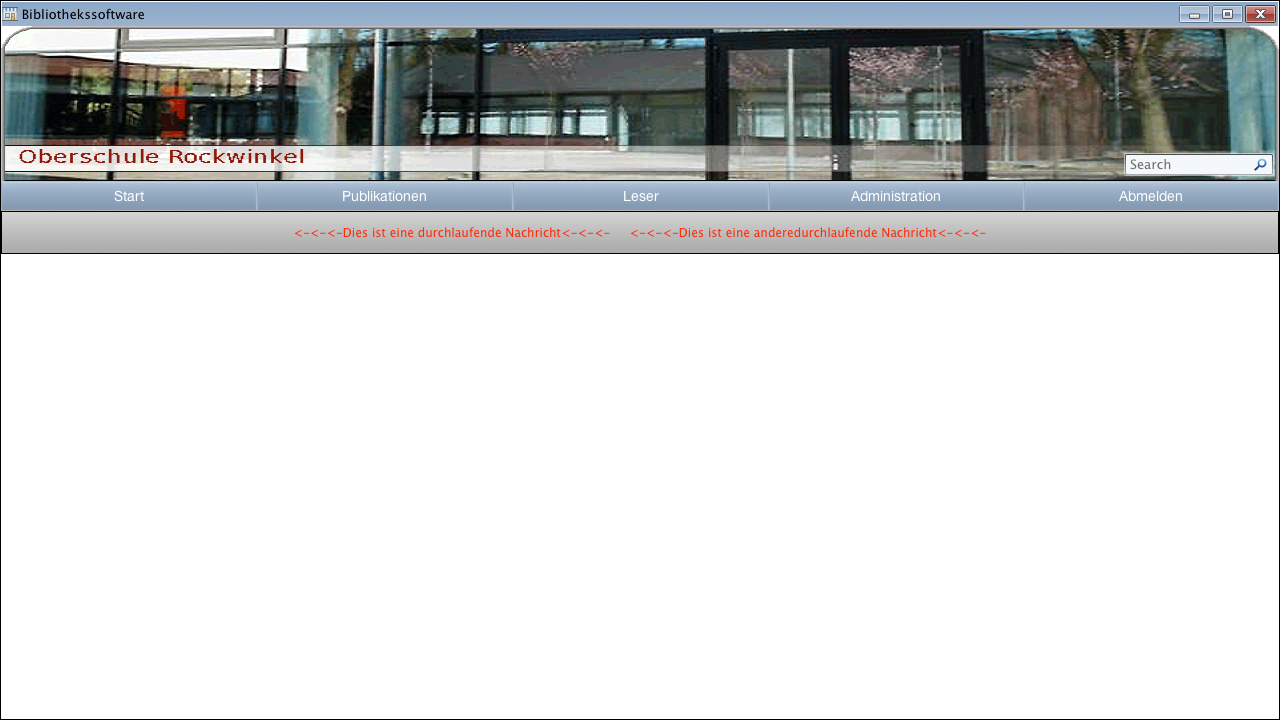
\includegraphics[width=1\textwidth]{WebApp-Screens/Startscreen-loggedIn.png}
  \label{startlog}
\end{figure}

\begin{table}[htbp]
\label{4}
\begin{tabular}{|l|p{10cm}|}
\hline 
\textbf{4} & \textbf{Startseite anzeigen} \\ \hline
\textbf{Akteure} & Bert Bib, Arnold Admin, Silke Schüler, Bart Besucher\\ \hline
\textbf{Ziel} & Der Akteur möchte die Startseite des Systems aufrufen  \\ \hline
\textbf{Vorbedingungen} & Das Programm wurde gestartet  \\ \hline
\textbf{Regulärer Ablauf} & 
1. Ein Benutzer drückt auf den Button 'Start' \\
&2. Das System zeigt die Startseite an\\
\hline
\textbf{Varianten} & 
Anwendungsfall 1 \\ \hline
\textbf{Nachbedingungen} & Es wird nun die Startseite angezeigt \\ \hline
\textbf{Fehler-/Ausnahmefälle} & keine\\
\hline
\end{tabular}
\end{table}

\begin{figure}[htbp]
\caption{Publikationsscreen von Silke Schüler oder Bart Besucher}
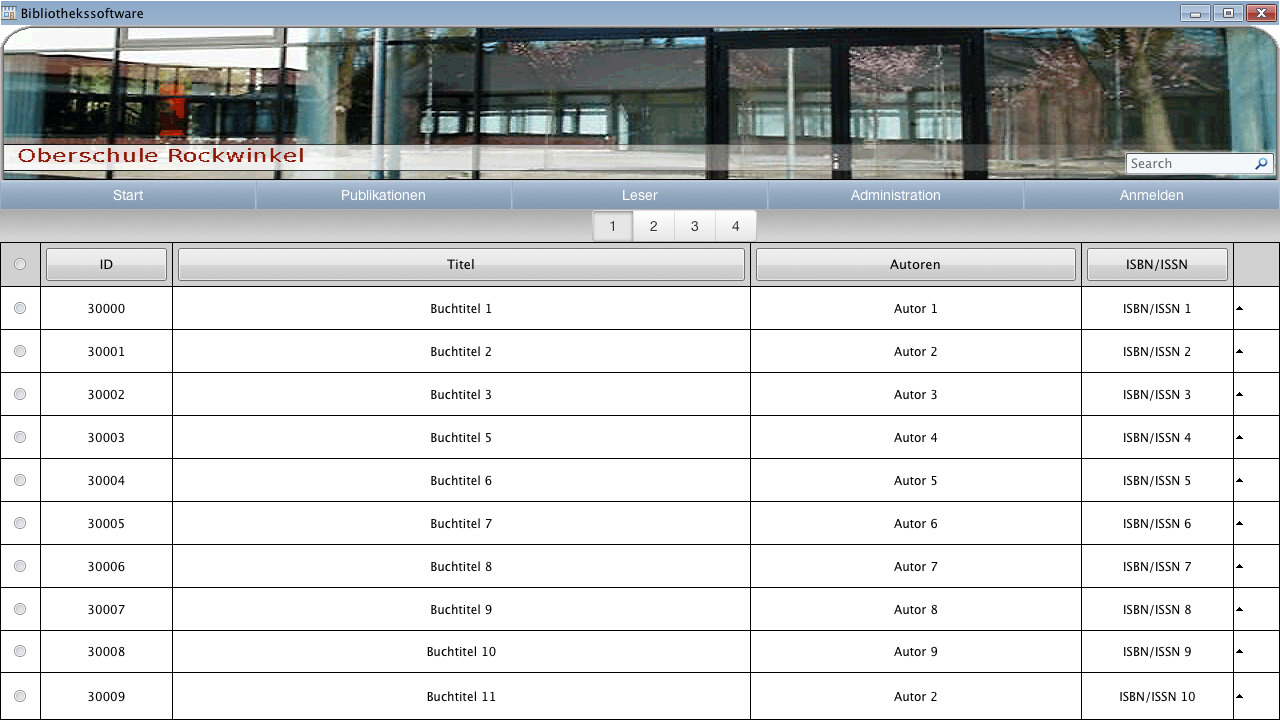
\includegraphics[width=1\textwidth]{WebApp-Screens/PublicationsscreenLogOut.png}
  \label{pub}
\end{figure}

\begin{table}[htbp]
\label{4.1}
\begin{tabular}{|l|p{10cm}|}
\hline 
\textbf{4.1} & \textbf{Leserprofil anzeigen} \\ \hline
\textbf{Akteure} & Silke Schüler\\ \hline
\textbf{Ziel} & Der Akteur möchte sich das eigene Leserprofil anzeigen lassen  \\ \hline
\textbf{Vorbedingungen} & Der Akteur ist angemeldet  \\ \hline
\textbf{Regulärer Ablauf} & 
1. Ein Benutzer drückt auf den Button 'Profil' \\
&2. Das System zeigt die Profilseite an\\
\hline
\textbf{Varianten} & 
keine \\ \hline
\textbf{Nachbedingungen} & Es wird nun die Profilseite angezeigt \\ \hline
\textbf{Fehler-/Ausnahmefälle} & keine\\
\hline
\end{tabular}
\end{table}

\begin{table}[htbp]
\label{4.1.1}
\begin{tabular}{|l|p{10cm}|}
\hline 
\textbf{4.1.1} & \textbf{Vormerkung bearbeiten} \\ \hline
\textbf{Akteure} & Silke Schüler\\ \hline
\textbf{Ziel} & Der Akteur möchte die eigenen Vormerkungen bearbeiten  \\ \hline
\textbf{Vorbedingungen} & Der Benutzer hat sein Profil geöffnet  \\ \hline
\textbf{Regulärer Ablauf} & 
1. Ein Benutzer drückt auf den Button 'Vormerkungen' \\
&2. Das System zeigt eine Liste der Vormerkungen an\\
\hline
\textbf{Varianten} & 
keine \\ \hline
\textbf{Nachbedingungen} & Es wird nun die Vormerkungen angezeigt, die bearbeitet werden können.\\ 
\hline
\textbf{Fehler-/Ausnahmefälle} & keine\\
\hline
\end{tabular}
\end{table}

\begin{table}[htbp]
\label{5}
\begin{tabular}{|l|p{10cm}|}
\hline 
\textbf{5} & \textbf{Publikationen anzeigen} \\ \hline
\textbf{Akteure} & Bert Bib, Arnold Admin, Silke Schüler, Bart Besucher\\ \hline
\textbf{Ziel} & Der Akteur möchte die Liste der Publikationen aufrufen  \\ \hline
\textbf{Vorbedingungen} & Das Programm wurde gestartet  \\ \hline
\textbf{Regulärer Ablauf} & 
1. Ein Benutzer drückt auf den Button 'Publikationen' \\
&2. Das System zeigt die Publikationsliste an\\
\hline
\textbf{Varianten} & 
keine \\ \hline
\textbf{Nachbedingungen} & Es wird nun die Liste mit den Publikationen angezeigt \\ \hline
\textbf{Fehler-/Ausnahmefälle} & keine\\
\hline
\end{tabular}
\end{table}

\begin{table}[htbp]
\label{6}
\begin{tabular}{|l|p{10cm}|}
\hline 
\textbf{6} & \textbf{Buch hinzufügen} \\ \hline
\textbf{Akteure} & Bert Bib\\ \hline
\textbf{Ziel} & Der Akteur möchte ein neues Buch hinzufügen \\ \hline
\textbf{Vorbedingungen} & Der Akteur ist als Bibliothekar angemeldet und hat die Publikationsliste 
aufgerufen  \\ \hline
\textbf{Regulärer Ablauf} & 
1. Der Benutzer drückt auf den Button 'Hinzufügen' \\
&2. Das System zeigt das Formular für das Hinzufügen eines Buches an\\
&3. Der Benutzer drückt den Button 'Speichern'\\
\hline
\textbf{Varianten} & 
keine \\ \hline
\textbf{Nachbedingungen} & Das Buch wurde gespeichert und ist in die Datenbank aufgenommen 
worden\\ \hline
\textbf{Fehler-/Ausnahmefälle} & 1. falsches ISBN-Format wurde eingeben\\
&2. Pflichtfelder wurden nicht eingegeben\\
\hline
\end{tabular}
\end{table}

\begin{table}[htbp]
\label{7}
\begin{tabular}{|l|p{10cm}|}
\hline 
\textbf{7} & \textbf{Buch ändern} \\ \hline
\textbf{Akteure} & Bert Bib\\ \hline
\textbf{Ziel} & Der Akteur möchte ein Daten eines Buches ändern \\ \hline
\textbf{Vorbedingungen} & Der Akteur ist als Bibliothekar angemeldet und hat die Detailsicht eines 
Buches aufgerufen  \\ \hline
\textbf{Regulärer Ablauf} & 
1. Der Benutzer drückt auf den Button 'Ändern' \\
&2. Das System zeigt das Formular für das Hinzufügen eines Buches an\\
&3. Der Benutzer drückt den Button 'Änderung speichern'\\
\hline
\textbf{Varianten} & 
keine \\ \hline
\textbf{Nachbedingungen} & Die Änderungen wurden gespeichert und sind in die Datenbank 
aufgenommen worden\\ \hline
\textbf{Fehler-/Ausnahmefälle} & 1. falsches ISBN-Format wurde eingeben\\
&2. Pflichtfelder wurden nicht eingegeben\\
\hline
\end{tabular}
\end{table}

\begin{table}[htbp]
\label{8}
\begin{tabular}{|l|p{10cm}|}
\hline 
\textbf{8} & \textbf{Buch löschen} \\ \hline
\textbf{Akteure} & Bert Bib\\ \hline
\textbf{Ziel} & Der Akteur möchte ein Buch löschen \\ \hline
\textbf{Vorbedingungen} & Der Akteur ist als Bibliothekar angemeldet und hat die Publikationsliste 
aufgerufen  \\ \hline
\textbf{Regulärer Ablauf} & 
1. Der Benutzer markiert die zu löschenden Bücher\\
&2. Der Benutzer drückt auf den Button 'Löschen' \\
\hline
\textbf{Varianten} & 
1. Der Benutzer befindet sich in der Detailsicht eines Buches\\
&2. Der Benutzer drückt auf den Button 'Löschen' \\ \hline
\textbf{Nachbedingungen} & Das Buch wurde gelöscht \\ \hline
\textbf{Fehler-/Ausnahmefälle} & \\
\hline
\end{tabular}
\end{table}

\begin{table}[htbp]
\label{9}
\begin{tabular}{|l|p{10cm}|}
\hline 
\textbf{9} & \textbf{CVS-Import} \\ \hline
\textbf{Akteure} & Bert Bib\\ \hline
\textbf{Ziel} & Der Akteur möchte eine CVS-Datei für Bücher importieren \\ \hline
\textbf{Vorbedingungen} & Der Akteur ist als Bibliothekar angemeldet und hat die Publikationsliste 
aufgerufen \\ \hline
\textbf{Regulärer Ablauf} & 
1. Der Benutzer drückt auf den Button CVS-Import \\
&2. Der Benutzer kann nun eine CVS-Datei auswählen\\
&3. Der Benutzer drückt den Button 'Importieren'\\
\hline
\textbf{Varianten} & 
keine \\ \hline
\textbf{Nachbedingungen} & Die CVS-Datei wurde hochgeladen und in der Datenbank ergänzt\\\hline
\textbf{Fehler-/Ausnahmefälle} & 1. falsches Datei-Format\\
\hline
\end{tabular}
\end{table}

\begin{table}[htbp]
\label{10}
\begin{tabular}{|l|p{10cm}|}
\hline 
\textbf{10} & \textbf{CVS-Export} \\ \hline
\textbf{Akteure} & Bert Bib\\ \hline
\textbf{Ziel} & Der Akteur möchte eine CVS-Datei von der Datenbank exportieren \\ \hline
\textbf{Vorbedingungen} & Der Akteur ist als Bibliothekar angemeldet und hat die Publikationsliste 
aufgerufen \\ \hline
\textbf{Regulärer Ablauf} & 
1. Der Benutzer drückt auf den Button CVS-Export \\
&2. Der Benutzer kann nun den Speicherort und Name für eine CVS-Datei auswählen\\
&3. Der Benutzer drückt den Button 'Exportieren'\\
\hline
\textbf{Varianten} & 
keine \\ \hline
\textbf{Nachbedingungen} & Die CVS-Datei wurde exportiert und gespeichert\\ \hline
\textbf{Fehler-/Ausnahmefälle} & keine\\
\hline
\end{tabular}
\end{table}

\begin{table}[htbp]
\label{11}
\begin{tabular}{|l|p{10cm}|}
\hline 
\textbf{11} & \textbf{Buch suchen} \\ \hline
\textbf{Akteure} & Bert Bib, Silke Schüler, Bart Besucher, Arnold Admin\\ \hline
\textbf{Ziel} & Der Akteur möchte ein Buch suchen \\ \hline
\textbf{Vorbedingungen} & keine \\ \hline
\textbf{Regulärer Ablauf} & 
1. Der Benutzer gibt den Suchbegriff in das Suchfeld ein und drückt 'Eingabe' \\
&2. Eine Liste von Büchern mit passendem Suchbegriff wird angezeigt\\
\hline
\textbf{Varianten} & 
keine \\ \hline
\textbf{Nachbedingungen} & Eine Liste von Büchern mit passendem Suchbegriff wird angezeigt\\ \hline
\textbf{Fehler-/Ausnahmefälle} & Zum eingegeben Suchbegriff existieren keine Daten\\
\hline
\end{tabular}
\end{table}

\begin{table}[htbp]
\label{12}
\begin{tabular}{|l|p{10cm}|}
\hline 
\textbf{12} & \textbf{Einzelnes Buch anzeigen/ Detailansicht} \\ \hline
\textbf{Akteure} & Bert Bib, Silke Schüler, Bart Besucher, Arnold Admin\\ \hline
\textbf{Ziel} & Der Akteur möchte sich Details zu einem Buch anzeigen lassen \\ \hline
\textbf{Vorbedingungen} & Die Publikationsliste oder die Suchliste wurde aufgerufen \\ \hline
\textbf{Regulärer Ablauf} & 
1. Der Benutzer klickt auf den Button 'Details' bei einem Buch in der Liste \\
&2. Die Detailseite des Buches wird angezeigt\\
\hline
\textbf{Varianten} & 
keine \\ \hline
\textbf{Nachbedingungen} & Die Detailseite eines Buches wird angezeigt\\ \hline
\textbf{Fehler-/Ausnahmefälle} & keine\\
\hline
\end{tabular}
\end{table}

\newpage

\begin{table}[htbp]
\label{13}
\begin{tabular}{|l|p{10cm}|}
\hline 
\textbf{13} & \textbf{Buch bewerten} \\ \hline
\textbf{Akteure} & Silke Schüler\\ \hline
\textbf{Ziel} & Der Akteur möchte ein Buch bewerten \\ \hline
\textbf{Vorbedingungen} & Die Detailansicht eines Buches wurde aufgerufen \\ \hline
\textbf{Regulärer Ablauf} & 
1. Der Benutzer klickt auf den Button 'Bewerten' und kann nun in einem Dropdownmenü eine Punktzahl 
auswählen\\
&2. Der Benutzer drückt den Button 'Buch bewerten'\\
\hline
\textbf{Varianten} & 
keine \\ \hline
\textbf{Nachbedingungen} & Das Buch wurde vom Akteur bewertet und lässt sich kein zweites Mal 
bewerten\\ \hline
\textbf{Fehler-/Ausnahmefälle} & Das Buch wurde schon einmal bewertet\\
\hline
\end{tabular}
\end{table}

\begin{table}[htbp]
\label{14}
\begin{tabular}{|l|p{10cm}|}
\hline 
\textbf{14} & \textbf{Buch ausleihen} \\ \hline
\textbf{Akteure} & Bert Bib, Silke Schüler\\ \hline
\textbf{Ziel} & Silke Schüler möchte ein Buch ausleihen \\ \hline
\textbf{Vorbedingungen} & Bert Bib ist im System als Bibliothekar angemeldet und Silke Schüler ist vor 
Ort \\ \hline
\textbf{Regulärer Ablauf} & 
1. Silke Schüler gibt Buch (Bücher) und ihren Bibliotheksausweis zum Einscannen an Bert Bib\\
&2. Bert Bib scannt erst den Ausweis\\
&3. Nun scannt Bert Bib die Bücher ein\\
&4. Die Liste der auszuleihenden Bücher wird mit dem Ausleiher angezeigt\\
&5. Bert Bib drückt auf den Button 'Ausleihen'\\
\hline
\textbf{Varianten} & 
keine \\ \hline
\textbf{Nachbedingungen} & Die Bücher stehen im System als 'ausgeliehen an Silke Schüler'\\ \hline
\textbf{Fehler-/Ausnahmefälle} & Silke Schüler ist gesperrt und kann keine Bücher ausleihen\\
\hline
\end{tabular}
\end{table}

\begin{table}[htbp]
\label{14.1}
\begin{tabular}{|l|p{10cm}|}
\hline 
\textbf{14.1} & \textbf{Buchrückgabe} \\ \hline
\textbf{Akteure} & Bert Bib, Silke Schüler\\ \hline
\textbf{Ziel} & Der Akteur will Bücher zurückgeben \\ \hline
\textbf{Vorbedingungen} & Bücher sind ausgeliehen \\ \hline
\textbf{Regulärer Ablauf} & 
1. Ein Akteur gibt abzugebene Bücher dem Bibliothekaren \\
&2. Der Bibliothekar scannt die Bücher ein\\
&3. Der Bibliothekar drückt auf den Button 'Bücher zurückgeben'\\
\hline
\textbf{Varianten} & 
Mahngebühren werden bezahlt \\ \hline
\textbf{Nachbedingungen} & Die Bücher stehen im System als zurückgegeben\\ \hline
\textbf{Fehler-/Ausnahmefälle} & keine\\
\hline
\end{tabular}
\end{table}

\begin{table}[htbp]
\label{14.1}
\begin{tabular}{|l|p{10cm}|}
\hline 
\textbf{14.1} & \textbf{Buchrückgabe} \\ \hline
\textbf{Akteure} & Bert Bib, Silke Schüler\\ \hline
\textbf{Ziel} & Der Akteur will Bücher zurückgeben \\ \hline
\textbf{Vorbedingungen} & Bücher sind ausgeliehen \\ \hline
\textbf{Regulärer Ablauf} & 
1. Ein Akteur gibt abzugebene Bücher dem Bibliothekaren \\
&2. Der Bibliothekar scannt die Bücher ein\\
&3. Der Bibliothekar drückt auf den Button 'Bücher zurückgeben'\\
\hline
\textbf{Varianten} & 
Mahngebühren werden bezahlt \\ \hline
\textbf{Nachbedingungen} & Die Bücher stehen im System als zurückgegeben\\ \hline
\textbf{Fehler-/Ausnahmefälle} & keine\\
\hline
\end{tabular}
\end{table}

\begin{table}[htbp]
\label{15}
\begin{tabular}{|l|p{10cm}|}
\hline 
\textbf{15} & \textbf{Buch rezensieren} \\ \hline
\textbf{Akteure} & Silke Schüler\\ \hline
\textbf{Ziel} & Der Akteur will ein Buch rezensieren \\ \hline
\textbf{Vorbedingungen} & Der Akteur befindet sich auf der Detailsicht eines Buches \\ \hline
\textbf{Regulärer Ablauf} & 
1. Der Akteur drückt auf 'Buch rezensieren' \\
&2. Der Akteur schreibt seine Rezension in das entsprechende Feld\\
&3. Der Button 'Rezension abschicken' wird gedrückt\\
\hline
\textbf{Varianten} & 
keine \\ \hline
\textbf{Nachbedingungen} & Die Rezension wird abgeschickt und der Bibliothekar muss diese nun 
freischalten\\ \hline
\textbf{Fehler-/Ausnahmefälle} & Es wurde nichts in das Bedienfeld eingegeben und dann abgeschickt.\\
\hline
\end{tabular}
\end{table}

\begin{table}[htbp]
\label{16}
\begin{tabular}{|l|p{10cm}|}
\hline 
\textbf{16} & \textbf{Buch vormerken} \\ \hline
\textbf{Akteure} & Silke Schüler\\ \hline
\textbf{Ziel} & Der Akteur will ein Buch vormerken \\ \hline
\textbf{Vorbedingungen} & Der Akteur befindet sich auf der Detailsicht eines Buches \\ \hline
\textbf{Regulärer Ablauf} & 
1. Der Akteur drückt auf 'Buch vormerken' \\
&2. Das Buch wurde vorgemerkt\\
\hline
\textbf{Varianten} & 
keine \\ \hline
\textbf{Nachbedingungen} & Das Buch wurde vorgemerkt und erscheint nun auf der Profilseite\\ \hline
\textbf{Fehler-/Ausnahmefälle} & Das Buch wurde bereits vorgemerkt und kann somit nicht noch einmal 
vorgemerkt werden\\
\hline
\end{tabular}
\end{table}

\begin{table}[htbp]
\label{17}
\begin{tabular}{|l|p{10cm}|}
\hline 
\textbf{17} & \textbf{Rezension freischalten} \\ \hline
\textbf{Akteure} & Bert Bib\\ \hline
\textbf{Ziel} & Der Bibliothekar will eine Rezension überprüfen und gegebenenfalls freischalten \\ \hline
\textbf{Vorbedingungen} & Es wurde eine Rezension geschrieben und der Bibliothekar hat diese zur 
Überprüfung erhalten. \\ \hline
\textbf{Regulärer Ablauf} & 
1. Der Akteur liest sich die Rezension durch \\
&2. Der Bibliothekar schaltet die Rezension frei\\
\hline
\textbf{Varianten} & 
1. Der Akteur ließt sich die Rezension durch \\
&2. Der Bibliothekar lehnt die Rezension ab \\ \hline
\textbf{Nachbedingungen} & Die Rezension wurde angenommen und freigeschaltet oder abgelehnt\\ 
\hline
\textbf{Fehler-/Ausnahmefälle} & \\
\hline
\end{tabular}
\end{table}

\begin{table}[htbp]
\label{18}
\begin{tabular}{|l|p{10cm}|}
\hline 
\textbf{18} & \textbf{Leserliste anzeigen} \\ \hline
\textbf{Akteure} & Bert Bib\\ \hline
\textbf{Ziel} & Der Akteur möchte die Liste der Leser aufrufen  \\ \hline
\textbf{Vorbedingungen} & Das Programm wurde gestartet  \\ \hline
\textbf{Regulärer Ablauf} & 
1. Ein Benutzer drückt auf den Button 'Leserliste' \\
&2. Das System zeigt die Leserliste an\\
\hline
\textbf{Varianten} & 
keine \\ \hline
\textbf{Nachbedingungen} & Es wird nun die Liste mit den Lesern angezeigt \\ \hline
\textbf{Fehler-/Ausnahmefälle} & keine\\
\hline
\end{tabular}
\end{table}

\begin{table}[htbp]
\label{19}
\begin{tabular}{|l|p{10cm}|}
\hline 
\textbf{19} & \textbf{Leser hinzufügen} \\ \hline
\textbf{Akteure} & Bert Bib\\ \hline
\textbf{Ziel} & Der Akteur möchte ein neuen Leser hinzufügen \\ \hline
\textbf{Vorbedingungen} & Der Akteur ist als Bibliothekar angemeldet und hat die Leserliste aufgerufen\\
\hline
\textbf{Regulärer Ablauf} & 
1. Der Benutzer drückt auf den Button 'Hinzufügen' \\
&2. Das System zeigt das Formular für das Hinzufügen eines Lesers an\\
&3. Der Bibliothekar füllt das Formular aus\\
&4. Der Benutzer drückt den Button 'Speichern'\\
\hline
\textbf{Varianten} & 
keine \\ \hline
\textbf{Nachbedingungen} & Der Leser wurde gespeichert und ist in die Datenbank aufgenommen 
worden\\ \hline
\textbf{Fehler-/Ausnahmefälle} & 1. Leser existiert bereits (alle Angaben stimmen überein)\\
&2. Pflichtfelder wurden nicht eingegeben\\
\hline
\end{tabular}
\end{table}

\begin{table}[htbp]
\label{20}
\begin{tabular}{|l|p{10cm}|}
\hline 
\textbf{20} & \textbf{Leser ändern} \\ \hline
\textbf{Akteure} & Bert Bib\\ \hline
\textbf{Ziel} & Der Akteur möchte die Daten eines Lesers ändern \\ \hline
\textbf{Vorbedingungen} & Der Akteur ist als Bibliothekar angemeldet und hat die Detailsicht eines 
Lesers aufgerufen  \\ \hline
\textbf{Regulärer Ablauf} & 
1. Der Benutzer drückt auf den Button 'Ändern' \\
&2. Das System zeigt das Formular für das Hinzufügen eines Lesers an\\
&3. Der Bibliothekar ändert das Formular entsprechend\\
&4. Der Benutzer drückt den Button 'Änderung speichern'\\
\hline
\textbf{Varianten} & 
keine \\ \hline
\textbf{Nachbedingungen} & Die Änderungen wurden gespeichert und sind in die Datenbank 
aufgenommen worden\\ \hline
\textbf{Fehler-/Ausnahmefälle} & 1. Leser existiert bereits\\
&2. Pflichtfelder wurden nicht eingegeben\\
\hline
\end{tabular}
\end{table}

\begin{table}[htbp]
\label{21}
\begin{tabular}{|l|p{10cm}|}
\hline 
\textbf{21} & \textbf{Leser löschen} \\ \hline
\textbf{Akteure} & Bert Bib\\ \hline
\textbf{Ziel} & Der Akteur möchte ein Leser löschen \\ \hline
\textbf{Vorbedingungen} & Der Akteur ist als Bibliothekar angemeldet und hat die Leserliste 
aufgerufen  \\ \hline
\textbf{Regulärer Ablauf} & 
1. Der Benutzer markiert die zu löschenden Leser\\
&2. Der Benutzer drückt auf den Button 'Löschen' \\
\hline
\textbf{Varianten} & 
1. Der Benutzer befindet sich in der Detailsicht eines Lesers\\
&2. Der Benutzer drückt auf den Button 'Löschen' \\ \hline
\textbf{Nachbedingungen} & Der Leser wurde gelöscht \\ \hline
\textbf{Fehler-/Ausnahmefälle} & \\
\hline
\end{tabular}
\end{table}

\begin{table}[htbp]
\label{22}
\begin{tabular}{|l|p{10cm}|}
\hline 
\textbf{22} & \textbf{CVS-Import} \\ \hline
\textbf{Akteure} & Bert Bib\\ \hline
\textbf{Ziel} & Der Akteur möchte eine CVS-Datei für Leser importieren \\ \hline
\textbf{Vorbedingungen} & Der Akteur ist als Bibliothekar angemeldet und hat die Leserliste aufgerufen\\
\hline
\textbf{Regulärer Ablauf} & 
1. Der Benutzer drückt auf den Button 'CVS-Import' \\
&2. Der Benutzer kann nun eine CVS-Datei auswählen\\
&3. Der Benutzer drückt den Button 'Importieren'\\
\hline
\textbf{Varianten} & 
keine \\ \hline
\textbf{Nachbedingungen} & Die CVS-Datei wurde hochgeladen und in der Datenbank ergänzt\\ \hline
\textbf{Fehler-/Ausnahmefälle} & 1. falsches Datei-Format\\
\hline
\end{tabular}
\end{table}

\begin{table}[htbp]
\label{23}
\begin{tabular}{|l|p{10cm}|}
\hline 
\textbf{23} & \textbf{CVS-Export} \\ \hline
\textbf{Akteure} & Bert Bib\\ \hline
\textbf{Ziel} & Der Akteur möchte eine CVS-Datei von der Datenbank exportieren \\ \hline
\textbf{Vorbedingungen} & Der Akteur ist als Bibliothekar angemeldet und hat die Leserliste 
aufgerufen \\ \hline
\textbf{Regulärer Ablauf} & 
1. Der Benutzer drückt auf den Button 'CVS-Export' \\
&2. Der Benutzer kann nun den Speicherort und Namen für eine CVS-Datei auswählen\\
&3. Der Benutzer drückt den Button 'Exportieren'\\
\hline
\textbf{Varianten} & 
keine \\ \hline
\textbf{Nachbedingungen} & Die CVS-Datei wurde exportiert und gespeichert\\ \hline
\textbf{Fehler-/Ausnahmefälle} & keine\\
\hline
\end{tabular}
\end{table}

\begin{table}[htbp]
\label{24}
\begin{tabular}{|l|p{10cm}|}
\hline 
\textbf{24} & \textbf{Einzelnen Leser anzeigen/ Detailansicht} \\ \hline
\textbf{Akteure} & Bert Bib\\ \hline
\textbf{Ziel} & Der Akteur möchte sich Details zu einem Leser anzeigen lassen \\ \hline
\textbf{Vorbedingungen} & Die Leserliste wurde aufgerufen \\ \hline
\textbf{Regulärer Ablauf} & 
1. Der Benutzer klickt auf den Button 'Details' bei einem Leser in der Liste \\
&2. Die Detailseite des Lesers wird angezeigt\\
\hline
\textbf{Varianten} & 
keine \\ \hline
\textbf{Nachbedingungen} & Die Detailseite eines Lesers wird angezeigt\\ \hline
\textbf{Fehler-/Ausnahmefälle} & keine\\
\hline
\end{tabular}
\end{table}

\begin{table}[htbp]
\label{24.1}
\begin{tabular}{|l|p{10cm}|}
\hline 
\textbf{24.1} & \textbf{Leser sperren} \\ \hline
\textbf{Akteure} & Bert Bib, Silke Schüler\\ \hline
\textbf{Ziel} & Der Bibliothekar sperrt einen Leser \\ \hline
\textbf{Vorbedingungen} & Die Detailsicht eines Lesers wurde aufgerufen \\ \hline
\textbf{Regulärer Ablauf} & 
1. Ein Leser gibt die ausgeliehenen nicht wieder zurück\\
&2. Der Bibliothekar sperrt den Nutzer\\
\hline
\textbf{Varianten} & 
1. Ein Leser verwendet seinen Account nicht ordnungsgemäß\\
&2. Der Bibliothekar sperrt den Nutzer\\ \hline
\textbf{Nachbedingungen} & Der Benutzer wurde gesperrt und kann keine Bücher mehr vormerken oder 
ausleihen\\ \hline
\textbf{Fehler-/Ausnahmefälle} & keine\\
\hline
\end{tabular}
\end{table}

\begin{table}[htbp]
\label{25}
\begin{tabular}{|l|p{10cm}|}
\hline 
\textbf{25} & \textbf{Leser suchen} \\ \hline
\textbf{Akteure} & Bert Bib\\ \hline
\textbf{Ziel} & Der Akteur möchte ein Leser suchen \\ \hline
\textbf{Vorbedingungen} & Die Leserliste wurde aufgerufen \\ \hline
\textbf{Regulärer Ablauf} & 
1. Der Bibliothekar gibt den Suchbegriff in das Suchfeld ein und drückt 'Eingabe' \\
&2. Eine Liste von Lesern mit passendem Suchbegriff wird angezeigt\\
\hline
\textbf{Varianten} & 
keine \\ \hline
\textbf{Nachbedingungen} & Eine Liste von Lesern mit passendem Suchbegriff wird angezeigt\\ \hline
\textbf{Fehler-/Ausnahmefälle} & Zum eingegeben Suchbegriff existieren keine Daten\\
\hline
\end{tabular}
\end{table}

\begin{table}[htbp]
\label{26}
\begin{tabular}{|l|p{10cm}|}
\hline 
\textbf{26} & \textbf{Administration öffnen} \\ \hline
\textbf{Akteure} & Bert Bib, Arnold Admin\\ \hline
\textbf{Ziel} & Der Akteur will die Administratorseite anzeigen lassen \\ \hline
\textbf{Vorbedingungen} & Der Akteur ist im System angemeldet \\ \hline
\textbf{Regulärer Ablauf} & 
1. Der Akteur klickt auf den Button 'Administration' \\
\hline
\textbf{Varianten} & 
keine \\ \hline
\textbf{Nachbedingungen} & Der Akteur befindet sich nun auf der Administrationsseite\\ \hline
\textbf{Fehler-/Ausnahmefälle} & keine\\
\hline
\end{tabular}
\end{table}

\newpage

\begin{table}[htbp]
\label{27}
\begin{tabular}{|l|p{10cm}|}
\hline 
\textbf{27} & \textbf{Bibliothekarliste anzeigen} \\ \hline
\textbf{Akteure} & Arnold Admin\\ \hline
\textbf{Ziel} & Der Akteur will die Liste der Bibliothekare einsehen \\ \hline
\textbf{Vorbedingungen} & Der Akteur ist im System angemeldet \\ \hline
\textbf{Regulärer Ablauf} & 
1. Der Akteur klickt auf den Button 'Administration' \\
&2. Der Akteur klickt auf den Button 'Bibliothekare'\\
\hline
\textbf{Varianten} & 
keine \\ \hline
\textbf{Nachbedingungen} & Der Akteur befindet sich nun auf der Seite, die Bibliothekare in einer 
Liste anzeigen\\ \hline
\textbf{Fehler-/Ausnahmefälle} & keine\\
\hline
\end{tabular}
\end{table}

\begin{table}[htbp]
\label{28}
\begin{tabular}{|l|p{10cm}|}
\hline 
\textbf{28} & \textbf{Bibliothekar hinzufügen} \\ \hline
\textbf{Akteure} & Arnold Admin\\ \hline
\textbf{Ziel} & Der Akteur will einen neuen Bibliothekaren hinzufügen \\ \hline
\textbf{Vorbedingungen} & Der Akteur ist als Admin angemeldet und hat die Bibliothekarsliste 
aufgerufen \\ \hline
\textbf{Regulärer Ablauf} & 
1. Der Akteur klickt auf den Button 'Hinzufügen' \\
&2. Der Admin füllt das Formular aus und klickt auf 'Speichern'\\
\hline
\textbf{Varianten} & 
keine \\ \hline
\textbf{Nachbedingungen} & Der Akteur befindet sich nun auf der Seite, die die Bibliothekarsliste 
anzeigt\\ \hline
\textbf{Fehler-/Ausnahmefälle} & keine\\
\hline
\end{tabular}
\end{table}


\begin{table}[htbp]
\label{29}
\begin{tabular}{|l|p{10cm}|}
\hline 
\textbf{29} & \textbf{Bibliothekar löschen} \\ \hline
\textbf{Akteure} & Arnold Admin\\ \hline
\textbf{Ziel} & Der Akteur will einen Bibliothekaren löschen \\ \hline
\textbf{Vorbedingungen} & Der Akteur ist als Admin angemeldet und hat die Bibliothekarsliste 
aufgerufen\\\hline
\textbf{Regulärer Ablauf} & 
1. Der Akteur klickt auf einen Bibliothekaren \\
&2. Der Admin klickt nun auf der Detailseite auf 'Löschen'\\
\hline
\textbf{Varianten} & 
keine \\ \hline
\textbf{Nachbedingungen} & Der Akteur befindet sich nun auf der Seite, die die Bibliothekarsliste 
anzeigt\\ \hline
\textbf{Fehler-/Ausnahmefälle} & keine\\
\hline
\end{tabular}
\end{table}

\begin{table}[htbp]
\label{30}
\begin{tabular}{|l|p{10cm}|}
\hline 
\textbf{30} & \textbf{Bibliothekar ändern} \\ \hline
\textbf{Akteure} & Arnold Admin\\ \hline
\textbf{Ziel} & Der Akteur will Daten eines Bibliothekaren ändern \\ \hline
\textbf{Vorbedingungen} & Der Akteur ist als Admin angemeldet und hat die Bibliothekarsliste 
aufgerufen \\ \hline
\textbf{Regulärer Ablauf} & 
1. Der Akteur klickt auf einen Bibliothekaren \\
&2. Der Akteur klickt auf der Detailseite auf 'Ändern '\\
&3. Der Akteur füllt das Formular aus und klickt auf 'Speichern'\\
\hline
\textbf{Varianten} & 
keine \\ \hline
\textbf{Nachbedingungen} & Der Akteur befindet sich nun auf der Seite, die die Bibliothekarliste 
anzeigt\\ \hline
\textbf{Fehler-/Ausnahmefälle} & keine\\
\hline
\end{tabular}
\end{table}


\begin{table}[htbp]
\label{31}
\begin{tabular}{|l|p{10cm}|}
\hline 
\textbf{31} & \textbf{Statistik anzeigen} \\ \hline
\textbf{Akteure} & Bert Bib\\ \hline
\textbf{Ziel} & Der Akteur will die Statistiken einsehen \\ \hline
\textbf{Vorbedingungen} & Der Akteur ist als Bibliothekar angemeldet und hat die Administrationsseite 
aufgerufen \\ \hline
\textbf{Regulärer Ablauf} & 
1. Der Akteur klickt auf den Button 'Statistiken' \\
\hline
\textbf{Varianten} & 
keine \\ \hline
\textbf{Nachbedingungen} & Der Akteur befindet sich nun auf der Seite, die die Statistiken anzeigt\\
\hline
\textbf{Fehler-/Ausnahmefälle} & keine\\
\hline
\end{tabular}
\end{table}


\begin{table}[htbp]
\label{32}
\begin{tabular}{|l|p{10cm}|}
\hline 
\textbf{32} & \textbf{Mahnungsliste anzeigen} \\ \hline
\textbf{Akteure} & Bert Bib\\ \hline
\textbf{Ziel} & Der Akteur will die Mahnungsliste einsehen \\ \hline
\textbf{Vorbedingungen} & Der Akteur ist als Bibliothekar angemeldet und hat die Administrationsseite 
aufgerufen \\ \hline
\textbf{Regulärer Ablauf} & 
1. Der Akteur klickt auf den Button 'Mahnungen' \\
\hline
\textbf{Varianten} & 
keine \\ \hline
\textbf{Nachbedingungen} & Der Akteur befindet sich nun auf der Seite, die die Mahnungsliste 
anzeigt\\ \hline
\textbf{Fehler-/Ausnahmefälle} & keine\\
\hline
\end{tabular}
\end{table}

\begin{table}[htbp]
\label{33}
\begin{tabular}{|l|p{10cm}|}
\hline 
\textbf{33} & \textbf{Mahnungsliste drucken} \\ \hline
\textbf{Akteure} & Bert Bib\\ \hline
\textbf{Ziel} & Der Akteur will die Mahnungsliste ausdrucken \\ \hline
\textbf{Vorbedingungen} & Der Akteur ist als Bibliothekar angemeldet und hat die Mahnungsliste 
aufgerufen \\ \hline
\textbf{Regulärer Ablauf} & 
1. Der Akteur klickt auf den Button 'Drucken' \\
\hline
\textbf{Varianten} & 
Einzelne Mahnungen werden ausgewählt damit nur diese ausgedruckt werden \\ \hline
\textbf{Nachbedingungen} & Der Akteur befindet sich nun auf der Seite, die die Mahnungsliste 
anzeigt\\ \hline
\textbf{Fehler-/Ausnahmefälle} & Probleme beim Drucken\\
\hline
\end{tabular}
\end{table}

\begin{table}[htbp]
\label{34}
\begin{tabular}{|l|p{10cm}|}
\hline 
\textbf{34} & \textbf{Mahnungsdetails anzeigen} \\ \hline
\textbf{Akteure} & Bert Bib\\ \hline
\textbf{Ziel} & Der Akteur will sich Details zu einer Mahnung anschauen \\ \hline
\textbf{Vorbedingungen} & Der Akteur ist als Bibliothekar angemeldet und hat die Mahnungsliste 
aufgerufen \\ \hline
\textbf{Regulärer Ablauf} & 
1. Der Akteur klickt auf eine Mahnung \\
\hline
\textbf{Varianten} & 
keine \\ \hline
\textbf{Nachbedingungen} & Der Akteur befindet sich nun auf der Seite, die die Mahnungsdetails 
anzeigt\\ \hline
\textbf{Fehler-/Ausnahmefälle} & keine\\
\hline
\end{tabular}
\end{table}

\begin{table}[htbp]
\label{35}
\begin{tabular}{|l|p{10cm}|}
\hline 
\textbf{35} & \textbf{Startseite bearbeiten} \\ \hline
\textbf{Akteure} & Bert Bib\\ \hline
\textbf{Ziel} & Der Akteur will die Startseite bearbeiten \\ \hline
\textbf{Vorbedingungen} & Der Akteur ist als Bibliothekar angemeldet und hat die 
Administrationsseite aufgerufen\\\hline
\textbf{Regulärer Ablauf} & 
1. Der Akteur klickt auf den Button 'Startseite bearbeiten' \\
&2. Der Akteur bearbeitet die Startseite nach seinen Wünschen und klickt auf 'Speichern'\\
\hline
\textbf{Varianten} & 
keine \\ \hline
\textbf{Nachbedingungen} & Der Akteur befindet sich nun auf der (neuen) Startseite \\ \hline
\textbf{Fehler-/Ausnahmefälle} & keine\\
\hline
\end{tabular}
\end{table}

\begin{table}[htbp]
\label{36}
\begin{tabular}{|l|p{10cm}|}
\hline 
\textbf{36} & \textbf{Abgabedaten und Mahngebühren bearbeiten} \\ \hline
\textbf{Akteure} & Bert Bib\\ \hline
\textbf{Ziel} & Der Akteur will Abgabedaten und Mahngebühren bearbeiten \\ \hline
\textbf{Vorbedingungen} & Der Akteur ist als Bibliothekar angemeldet und hat die Administrationsseite 
aufgerufen \\ \hline
\textbf{Regulärer Ablauf} & 
1. Der Akteur klickt auf den Button 'Abgabedaten/Mahngebühren bearbeiten' \\
&2. Der Akteur bearbeitet die Daten und/oder Gebühren und klickt auf 'Speichern'\\
\hline
\textbf{Varianten} & 
keine \\ \hline
\textbf{Nachbedingungen} & Der Akteur befindet sich auf der gleichen Seite und kann die neuen 
Daten/Gebühren sehen\\ \hline
\textbf{Fehler-/Ausnahmefälle} & keine\\
\hline
\end{tabular}
\end{table}

\newpage
\subsection{Aktionen}
  {\em Hier sollten die gleichen Aktionen wie in den Anwendungsfällen
  genannt und genauer beschrieben werden. Mit anderen Worten: Die
  Anwendungsfälle müssen vollständig durch Ausführung von Aktionen aus
  dieser Liste durchführbar sein. Im Prinzip muss es z.B.\ für jeden
  Button/Menüpunkt/Link eine Aktion geben. Dabei ist zu beachten:
  \begin{itemize}
    \item Die Namen sollten sinnvoll und eindeutig sein.

    \item Die Parameter der Aktionen sollen angegeben werden. Hier
    sollen sprechende Namen verwendet werden. Eventuell müssen die
    Parameter auch genauer erläutert werden.

    \item Es müssen maximale Ausführungszeiten für jede Operation
    angegeben werden.
    
  \item Die Gruppierung und Sortierung sollte sinnvoll sein
    (z.B. alphabetisch).
  \end{itemize}

  Wenn Ihr z.B.\ irgendwo in Eurer GUI ein Suchfeld habt, in das Ihr
  den Namen eines Kunden eintragen könnt, und einen Button, welcher die
  Suche startet, dann wird es vermutlich eine Aktion {\bf Kunde
    suchen(name)} geben. Dies ist eine Funktion, die Euer System
  bereitstellt und die durch Anklicken des Buttons ausgelöst wird. Der
  Anwendungsfall {\bf Kunde suchen} verwendet dann diese Aktion,
  enthält aber zusätzlich die Beschreibung der Interaktion mit dem
  System.
  
  Dieser Abschnitt ist im Standard im Prinzip vorgesehen, weil hierzu
  grundsätzlich eine Aussage gemacht werden muss. Die Aktionen sind
  letztlich die Produktfunktionen, während die Anwendungsfälle die
  Interaktion zwischen Akteuren und System beschreiben. }

  \begin{table}[htbp]
  \label{a1}
  \begin{tabular}{|l|p{10cm}|}
  \hline 
  \textbf{1} & \textbf{Abgabedaten bearbeiten(zeitraum)} \\ \hline
  \textbf{Beschreibung} & Hier kann der Bibliothekar die Abgabedaten eines Buches bearbeiten\\ \hline
  \textbf{Parameter} & Der Zeitraum, wie lange ein Buch ausgeliehen werden darf\\ \hline
  \textbf{Ausführungszeit} & 1s\\ \hline
  \end{tabular}
  \end{table}
  
  \begin{table}[htbp]
  \label{a2}
  \begin{tabular}{|l|p{10cm}|}
  \hline 
  \textbf{2} & \textbf{Abmelden} \\ \hline
  \textbf{Beschreibung} & Über den Button meldet sich der Nutzer ab\\ \hline
  \textbf{Parameter} & keine \\ \hline
  \textbf{Ausführungszeit} & 1s\\ \hline
  \end{tabular}
  \end{table}
  
  \begin{table}[htbp]
  \label{a3}
  \begin{tabular}{|l|p{10cm}|}
  \hline 
  \textbf{3} & \textbf{Administration öffnen} \\ \hline
  \textbf{Beschreibung} & Die Seite der Administration öffnet sich und alle Funktionen erscheinen\\ \hline
  \textbf{Parameter} & keine \\ \hline
  \textbf{Ausführungszeit} & 2s\\ \hline
  \end{tabular}
  \end{table}
  
  \begin{table}[htbp]
  \label{a4}
  \begin{tabular}{|l|p{10cm}|}
  \hline 
  \textbf{4} & \textbf{Anmelden(name, passwort)} \\ \hline
  \textbf{Beschreibung} & Der Nutzer meldet sich im System an und hat nun alle Zugriffsrechte die ihm zustehen\\ \hline
  \textbf{Parameter} & Der Nutzername und das entsprechende Passwort \\ \hline
  \textbf{Ausführungszeit} & 3s\\ \hline
  \end{tabular}
  \end{table}
  
    \begin{table}[htbp]
    \label{a5}
    \begin{tabular}{|l|p{10cm}|}
    \hline 
    \textbf{5} & \textbf{Bibliothekar ändern(daten)} \\ \hline
    \textbf{Beschreibung} & Der Administrator ändert die Daten eines Bibliothekars\\ \hline
    \textbf{Parameter} & Die neuen Daten des Bibliothekars \\ \hline
    \textbf{Ausführungszeit} & 2s\\ \hline
    \end{tabular}
    \end{table}
  
\begin{table}[htbp]
    \label{a6}
    \begin{tabular}{|l|p{10cm}|}
    \hline 
    \textbf{6} & \textbf{Bibliothekar hinzufügen(daten)} \\ \hline
    \textbf{Beschreibung} & Der Administrator fügt einen Bibliothekar hinzu\\ \hline
    \textbf{Parameter} & Die Daten des Bibliothekars \\ \hline
    \textbf{Ausführungszeit} & 2s\\ \hline
    \end{tabular}
    \end{table}
    
  \begin{table}[htbp]
  \label{a7}
  \begin{tabular}{|l|p{10cm}|}
  \hline 
  \textbf{7} & \textbf{Bibliothekar löschen} \\ \hline
  \textbf{Beschreibung} & Der Administrator löscht einen bestehenden Bibliothekar\\ \hline
  \textbf{Parameter} & keine \\ \hline
  \textbf{Ausführungszeit} & 2s\\ \hline
  \end{tabular}
  \end{table}

  \begin{table}[htbp]
  \label{a8}
  \begin{tabular}{|l|p{10cm}|}
  \hline 
  \textbf{8} & \textbf{Bibliothekarsliste anzeigen} \\ \hline
  \textbf{Beschreibung} & Die Liste der Bibliothekare wird angezeigt\\ \hline
  \textbf{Parameter} & keine \\ \hline
  \textbf{Ausführungszeit} & 2s\\ \hline
  \end{tabular}
  \end{table}

  \begin{table}[htbp]
  \label{a9}
  \begin{tabular}{|l|p{10cm}|}
  \hline 
  \textbf{9} & \textbf{Buch ändern(daten)} \\ \hline
  \textbf{Beschreibung} & Ein vorhandenes Buch wird verändert \\ \hline
  \textbf{Parameter} & Die neuen Daten des Buches \\ \hline
  \textbf{Ausführungszeit} & 2s\\ \hline
  \end{tabular}
  \end{table}

  \begin{table}[htbp]
  \label{a10}
  \begin{tabular}{|l|p{10cm}|}
  \hline 
  \textbf{10} & \textbf{ Buch ausleihen(buch)} \\ \hline
  \textbf{Beschreibung} & Ein Buch wird von einem Nutzer ausgeliehen und über einem Scanner erkannt \\ \hline
  \textbf{Parameter} & Das Buch welches ausgeliehen werden soll \\ \hline
  \textbf{Ausführungszeit} & 4s\\ \hline
  \end{tabular}
  \end{table}

  \begin{table}[htbp]
  \label{a11}
  \begin{tabular}{|l|p{10cm}|}
  \hline 
  \textbf{11} & \textbf{Buch bewerten(wertung)} \\ \hline
  \textbf{Beschreibung} & Ein Buch wird von einem Nutzer bewertet\\ \hline
  \textbf{Parameter} & Die Anzahl der Punkte die das Buch bekommen soll \\ \hline
  \textbf{Ausführungszeit} & 1s\\ \hline
  \end{tabular}
  \end{table}

  \begin{table}[htbp]
  \label{a12}
  \begin{tabular}{|l|p{10cm}|}
  \hline 
  \textbf{12} & \textbf{Buch hinzufügen(daten)} \\ \hline
  \textbf{Beschreibung} & Ein Buch wird in die Datenbank hinzugefügt\\ \hline
  \textbf{Parameter} & Die Daten des neuen Buches \\ \hline
  \textbf{Ausführungszeit} & 2s\\ \hline
  \end{tabular}
  \end{table}

  \begin{table}[htbp]
  \label{a13}
  \begin{tabular}{|l|p{10cm}|}
  \hline 
  \textbf{13} & \textbf{Buch löschen()} \\ \hline
  \textbf{Beschreibung} & Ein Buch wird aus der Datenbank gelöscht\\ \hline
  \textbf{Parameter} & keine \\ \hline
  \textbf{Ausführungszeit} & 1s\\ \hline
  \end{tabular}
  \end{table}

  \begin{table}[htbp]
  \label{a14}
  \begin{tabular}{|l|p{10cm}|}
  \hline 
  \textbf{14} & \textbf{Buch rezensieren(buch)} \\ \hline
  \textbf{Beschreibung} & Eine Rezension über ein Buch wird geschrieben\\ \hline
  \textbf{Parameter} & Das Buch über welches die Rezension verfasst wird \\ \hline
  \textbf{Ausführungszeit} & 2s\\ \hline
  \end{tabular}
  \end{table}

  \begin{table}[htbp]
  \label{a15}
  \begin{tabular}{|l|p{10cm}|}
  \hline 
  \textbf{15} & \textbf{Buch suchen(buch)} \\ \hline
  \textbf{Beschreibung} & Ein Buch wird in der Datenbank gesucht\\ \hline
  \textbf{Parameter} & Der Name des Buches, welches gesucht wird \\ \hline
  \textbf{Ausführungszeit} & 2s\\ \hline
  \end{tabular}
  \end{table}


  \begin{table}[htbp]
  \label{a16}
  \begin{tabular}{|l|p{10cm}|}
  \hline 
  \textbf{16} & \textbf{Buch vormerken(buch)} \\ \hline
  \textbf{Beschreibung} & Ein Buch wird von einem Nutzer vorgemerkt\\ \hline
  \textbf{Parameter} & Das Buch, welches vorgemerkt werden soll \\ \hline
  \textbf{Ausführungszeit} & 1s\\ \hline
  \end{tabular}
  \end{table}


  \begin{table}[htbp]
  \label{a17}
  \begin{tabular}{|l|p{10cm}|}
  \hline 
  \textbf{17} & \textbf{Buchrückgabe(buch)} \\ \hline
  \textbf{Beschreibung} & Ein Buch wird von einem Nutzer zurückgegeben\\ \hline
  \textbf{Parameter} & Das Buch, welches zurück gegeben werden soll \\ \hline
  \textbf{Ausführungszeit} & 4s\\ \hline
  \end{tabular}
  \end{table}

  \begin{table}[htbp]
  \label{a18}
  \begin{tabular}{|l|p{10cm}|}
  \hline 
  \textbf{18} & \textbf{CVS-Import(datei)} \\ \hline
  \textbf{Beschreibung} & Eine CVS-Datei wird importiert und die Daten werden in die Datenbank geschrieben\\ \hline
  \textbf{Parameter} & Die CVS-Datei, welche importiert werden soll \\ \hline
  \textbf{Ausführungszeit} & Abhängig von der Größe der Datei(ca. 4-15s)\\ \hline
  \end{tabular}
  \end{table}

\newpage

  \begin{table}[htbp]
  \label{a19}
  \begin{tabular}{|l|p{10cm}|}
  \hline 
  \textbf{19} & \textbf{CVS-Export(liste)} \\ \hline
  \textbf{Beschreibung} & Eine CVS-Datei wird exportiert und die Daten werden in eine CVS-Datei gespeichert\\ \hline
  \textbf{Parameter} & Die Liste der Bücher oder Leser, welche gespeichert werden soll \\ \hline
  \textbf{Ausführungszeit} & Abhängig von der Größe der Liste(ca. 4-15s)\\ \hline
  \end{tabular}
  \end{table}

  \begin{table}[htbp]
  \label{a20}
  \begin{tabular}{|l|p{10cm}|}
  \hline 
  \textbf{20} & \textbf{Einzelnes Buch anzeigen/ Detailansicht()} \\ \hline
  \textbf{Beschreibung} & Ein ausgewähltes Buch soll im Detail angezeigt werden\\ \hline
  \textbf{Parameter} & keine \\ \hline
  \textbf{Ausführungszeit} & 1s\\ \hline
  \end{tabular}
  \end{table}

  \begin{table}[htbp]
  \label{a21}
  \begin{tabular}{|l|p{10cm}|}
  \hline 
  \textbf{21} & \textbf{Leser ändern(daten)} \\ \hline
  \textbf{Beschreibung} & Die Daten eines Lesers werden verändert\\ \hline
  \textbf{Parameter} & Die aktuellen Daten des Lesers \\ \hline
  \textbf{Ausführungszeit} & 2s\\ \hline
  \end{tabular}
  \end{table}

  \begin{table}[htbp]
  \label{a22}
  \begin{tabular}{|l|p{10cm}|}
  \hline 
  \textbf{22} & \textbf{Leser hinzufügen(daten)} \\ \hline
  \textbf{Beschreibung} & Ein Leser wird neu registriert und hinzugefügt\\ \hline
  \textbf{Parameter} & Die Daten des neuen Lesers \\ \hline
  \textbf{Ausführungszeit} & 2s\\ \hline
  \end{tabular}
  \end{table}


  \begin{table}[htbp]
  \label{a23}
  \begin{tabular}{|l|p{10cm}|}
  \hline 
  \textbf{23} & \textbf{Leser löschen(leser)} \\ \hline
  \textbf{Beschreibung} & Ein Leser wird aus der Datenbank gelöscht\\ \hline
  \textbf{Parameter} & Der Leser, welcher gelöscht werden soll \\ \hline
  \textbf{Ausführungszeit} & 1s\\ \hline
  \end{tabular}
  \end{table}

  \begin{table}[htbp]
  \label{a24}
  \begin{tabular}{|l|p{10cm}|}
  \hline 
  \textbf{24} & \textbf{Leser sperren(leser)} \\ \hline
  \textbf{Beschreibung} & Ein Leser wird gesperrt und kann so kein Buch mehr ausleihen\\ \hline
  \textbf{Parameter} & Der Leser, welcher gesperrt werden soll \\ \hline
  \textbf{Ausführungszeit} & 1s\\ \hline
  \end{tabular}
  \end{table}

  \begin{table}[htbp]
  \label{a25}
  \begin{tabular}{|l|p{10cm}|}
  \hline 
  \textbf{25} & \textbf{Leser suchen(name)} \\ \hline
  \textbf{Beschreibung} & Ein Leser wird im System gesucht\\ \hline
  \textbf{Parameter} & Der Name des Lesers, welcher gesucht wird \\ \hline
  \textbf{Ausführungszeit} & 2s\\ \hline
  \end{tabular}
  \end{table}

  \begin{table}[htbp]
  \label{a26}
  \begin{tabular}{|l|p{10cm}|}
  \hline 
  \textbf{26} & \textbf{Leserliste anzeigen()} \\ \hline
  \textbf{Beschreibung} & Die Liste aller Leser wird angezeigt\\ \hline
  \textbf{Parameter} & keine \\ \hline
  \textbf{Ausführungszeit} & 2s\\ \hline
  \end{tabular}
  \end{table}


  \begin{table}[htbp]
  \label{a27}
  \begin{tabular}{|l|p{10cm}|}
  \hline 
  \textbf{27} & \textbf{Leserprofil anzeigen()} \\ \hline
  \textbf{Beschreibung} & Ein Leser lässt sich sein eigenes Profil anzeigen\\ \hline
  \textbf{Parameter} & keine \\ \hline
  \textbf{Ausführungszeit} & 2s\\ \hline
  \end{tabular}
  \end{table}

  \begin{table}[htbp]
  \label{a28}
  \begin{tabular}{|l|p{10cm}|}
  \hline 
  \textbf{28} & \textbf{Mahngebühr ändern(gebühr,buch)} \\ \hline
  \textbf{Beschreibung} & Der Bibliothekar ändert die Gebühr eines Buches\\ \hline
  \textbf{Parameter} & Die neue Gebühr die nun anfällt und das Buch, welches die neue Gebühr erhalten soll \\ \hline
  \textbf{Ausführungszeit} & 1s\\ \hline
  \end{tabular}
  \end{table}
  
  
  \begin{table}[htbp]
  \label{a29}
  \begin{tabular}{|l|p{10cm}|}
  \hline 
  \textbf{29} & \textbf{Mahnungsdetails anzeigen(mahnung)} \\ \hline
  \textbf{Beschreibung} & Die Details einer Mahnung werden angezeigt\\ \hline
  \textbf{Parameter} & Die Mahnung, welche angezeigt werden soll \\ \hline
  \textbf{Ausführungszeit} & 1s\\ \hline
  \end{tabular}
  \end{table}

  \begin{table}[htbp]
  \label{a30}
  \begin{tabular}{|l|p{10cm}|}
  \hline 
  \textbf{30} & \textbf{Mahnungsliste anzeigen()} \\ \hline
  \textbf{Beschreibung} & Die Liste der Mahnungen wird angezeigt\\ \hline
  \textbf{Parameter} & keine \\ \hline
  \textbf{Ausführungszeit} & 2s\\ \hline
  \end{tabular}
  \end{table}

  \begin{table}[htbp]
  \label{a31}
  \begin{tabular}{|l|p{10cm}|}
  \hline 
  \textbf{31} & \textbf{Mahnungsliste drucken()} \\ \hline
  \textbf{Beschreibung} & Die Liste der Mahnungen wird gedruckt\\ \hline
  \textbf{Parameter} & keine \\ \hline
  \textbf{Ausführungszeit} & Abhängig von der Größe der Liste und Verbindung zu Drucker(ca. 5-20s)\\ \hline
  \end{tabular}
  \end{table}

  \begin{table}[htbp]
  \label{a32}
  \begin{tabular}{|l|p{10cm}|}
  \hline 
  \textbf{32} & \textbf{Publikationen anzeigen()} \\ \hline
  \textbf{Beschreibung} & Die Liste der Publikationen wird angezeigt\\ \hline
  \textbf{Parameter} & keine \\ \hline
  \textbf{Ausführungszeit} & 2s\\ \hline
  \end{tabular}
  \end{table}

  \begin{table}[htbp]
  \label{a33}
  \begin{tabular}{|l|p{10cm}|}
  \hline 
  \textbf{33} & \textbf{Rezension freischalten()} \\ \hline
  \textbf{Beschreibung} & Eine geschriebene Rezension wird überprüft und freigeschaltet\\ \hline
  \textbf{Parameter} & keine \\ \hline
  \textbf{Ausführungszeit} & 1s\\ \hline
  \end{tabular}
  \end{table}

  \begin{table}[htbp]
  \label{a34}
  \begin{tabular}{|l|p{10cm}|}
  \hline 
  \textbf{34} & \textbf{Start anzeigen()} \\ \hline
  \textbf{Beschreibung} & Die Startseite wird angezeigt\\ \hline
  \textbf{Parameter} & keine \\ \hline
  \textbf{Ausführungszeit} & 2s\\ \hline
  \end{tabular}
  \end{table}

  \begin{table}[htbp]
  \label{a35}
  \begin{tabular}{|l|p{10cm}|}
  \hline 
  \textbf{35} & \textbf{Startseite bearbeiten(text)} \\ \hline
  \textbf{Beschreibung} & Die Startseite wird bearbeitet\\ \hline
  \textbf{Parameter} & Der Text der nun auf der Startseite erscheinen soll \\ \hline
  \textbf{Ausführungszeit} & 2s\\ \hline
  \end{tabular}
  \end{table}

  \begin{table}[htbp]
  \label{a36}
  \begin{tabular}{|l|p{10cm}|}
  \hline 
  \textbf{36} & \textbf{Statistiken anzeigen()} \\ \hline
  \textbf{Beschreibung} & Die Statistiken werden angezeigt\\ \hline
  \textbf{Parameter} & keine \\ \hline
  \textbf{Ausführungszeit} & 2s\\ \hline
  \end{tabular}
  \end{table}
  
\subsection{Entwurfseinschränkungen}
\nurlangversion

{\em Wurde bereits in \ref{sec:Einschraenkungen} behandelt und muss
  daher hier nicht wiederholt werden. Falls aber eine detailliertere
  Beschreibung notwendig wäre, wäre hier der geeignete Ort.}
  

\subsection{Softwaresystemattribute}
  {\em Hier werden die sogenannten „nichtfunktionalen Anforderungen“
  spezifiziert. Dazu gehören beispielsweise:
  \begin{itemize}
    \item Performanz:
    \item Zuverlässigkeit (Korrektheit, Robustheit, Ausfallsicherheit):
    \item Verfügbarkeit:
    \item Sicherheit:
     Sicherheit bezüglich der persönlichen Daten wird zum Teil durch den 
     passwortgeschützten Login gewährleistet, wobei jeder Nutzer ein individuelles 
     Passwort besitzt. Auf Profildaten haben nur der bestimmte eingeloggte          
     Leser und die Mitarbeiter Zugriff. Zusätzlich werden vor dem Versenden von Daten, 
     diese via SSL verschlüsselt, was die Datensicherheit in unserem System 
     garantiert.
    \item Wartbarkeit:
    
    \item Portabilität:
    
  \end{itemize}
}

{\em Die spezifizierten Systemattribute müssen hinreichend konkret und
  überprüfbar formuliert werden.}



\subsection{Weitere Anforderungen}
\nurlangversion

{\em In diesem Abschnitt können weitere relevante Anforderungen
  beschrieben werden, die in keine der oben genannten Abschnitte
  passen.}

\section{Anhang}
\nurlangversion

{\em Hier können weitere detailliertere Ergebnisse aus der Ist-Analyse
  oder andere Informationen, die zur Erstellung der Spezifikation
  gedient haben (z.B. Papierprototypen), angefügt werden.}

\end{document}
